\documentclass{article}
\usepackage[utf8]{inputenc}
\usepackage{hyperref}
\usepackage{algorithm}
\usepackage{algorithmicx}
\usepackage[table]{xcolor}
\usepackage{algpseudocode}
\usepackage{authblk}
\usepackage{graphicx}
\usepackage[margin=0.70in]{geometry}
\usepackage{listings}
\usepackage{indentfirst}

\title{Homework 2-1: Parallelizing a Particle Simulation with OpenMP}
\author{Andrew Chen}
\author{Xuan Jiang}
\author{Brian Park}
\affil{UC Berkeley, Computer Science 267}
\date{February 2022}

\begin{document}

\maketitle
\section{Introduction}
We used variety of techniques to optimize the problem of parallelizing $n$-body particle simulation on the Cori KNL node. In the remainder of this report, we describe each of our optimizations in our final submission, present experimental results, and describe attempted optimizations worked and did not work. We first accelerated particle simulation from $O(n^2)$ to $O(n)$ serially on a single core/thread. Then we parallelized our $O(n)$ solution using OpenMP (Open Multi-Processing) \cite{openmp}.

\section{Serial}

\subsection{Data Structures}
We defined our bins as vectors:

\begin{itemize}
    \item \verb|vector<particle_t*> bin_t| \\
        This holds pointers to all of the particles that lie within a bin.
    \item \verb|bin_t* bins| \\
        This holds the vector of bins stored in row-major order.
\end{itemize}

We make sure that particles are stored in bins. The number of bins is fixed which is why we use an array of bins. The bins themselves change in size at each simulation step when they move around, which is why we use \verb|std::vector|. Note that \verb|std::vector| is not thread-safe, so we need to implement the synchronization ourselves, which OpenMP directives conveniently provide.

\subsection{Design Choice}
For the serial runtime code, we optimized the algorithm to be run $O(n^2)$ to $O(n)$. The way we cut down this runtime was by first doing particle binning. Since there is a threshold cutoff radius of how far two particles need to be to apply force on each other determined by \verb|r2 <= cutoff * cutoff|, we can partition the dataset into bins. That way, we can call \verb|apply_force| on a particle on its neighboring bins, avoiding wasteful iterations on the whole working dataset. We need to look in neighboring bins since a particle could lie on the edge of a bin and it could interact with a particle in a neighboring bin. First we optimized this by applying force and updating acceleration on eight neighboring bins of a particular bin, along with the bin itself. This brought us a speed of 2392.5 seconds for 1000000 particles.

We can even do a further optimization and cut the number of total iterations by nearly half. We first did iterations of neighboring bins on each bin in row-major order. Since force is applied and exerted on both particles, we can actually do two redundant computations at once. With that, that also requires a modification that only needs to compare four neighboring bins (right, lower left, lower, lower right). This brought our time even lower to 1629.9 seconds.

A similar optimization can be done when applying force to particles within one bin (ignoring neighboring bins). By applying force in pairs, and making sure to iterate over unique pairs of particles, iterations can be cut in half.

At this moment, our bins were represented by a $2D$ vector. However, we did not need the number of bins to be dynamic, and we switched our bins representation to be an array of vectors. This further brought the time from 1629.9 to 1413.9 seconds.

Our implementation at this point also had inefficient memory management. For each \verb|simulate_one_step()|, we would set \verb|bins = new bin_t[grid_size * grid_size]| in order to clear out the bin vectors to prepare for the next simulation. Although there are no loops, it turns out that this method of clearing all the vectors was slower than going through each vector and calling \verb|vector.clear()| due to the overhead of deleting and re-mallocing a large array each simulation. Finally, the clearing of the bins could be done immediately after applying the forces within the bin, so there did not need to be a dedicated for loop for clearing. Combined with other small changes such as using the stack instead of the heap where possible, passing by pointer instead of by value, time was reduced from 1413.9 seconds to 876.9s.

\section{OpenMP}
\subsection{Design Choice}
As OpenMP uses the fork-join model, we had to make sure to parallelize and minimize serialized code as much as possible. We tried to separate the code into several sections, and use \verb|#pragma omp master| for every section and change them one by one to \verb|#pragma omp for| to parallelize it. Then we implemented locks while updating bins, which is necessary since the \verb|std::vector| class is not thread-safe in a multi-threaded context. We also need a \verb|#pragma omp barrier| before and after \verb|binning()| since we refresh the bins at each iteration. Note that there is an implicit barrier after the end of every \verb|#pragma omp for|, but we still provide an explicit barrier. This is because we need to refresh bins per every iteration, and \verb|simulate_one_step()| is already in a parallel context in \verb|main.cpp|. Barriers just ensure our data in bins is correct before and after the end of each iteration. Although adding more synchronization hurt our performance more, the trade off is necessary to prevent incorrect results.

\subsection{Synchronization}
The first issue in parallelism with OpenMP was WAW (write after write) hazards. Multiple threads share the same main memory, and we also noticed that some threads were trying to update the same memory location. To circumvent this, OpenMP synchronization primitives are needed to make sure variables are thread-safe and not prone to any data hazards. We used locks to protect data attributes via \verb|omp_set_lock| and \verb|omp_unset_lock|. Doing this will prevent any data races. We believe that these are the minimal amount of synchronizations needed for protecting data, no need for conditional variables or semaphores. We could've also used OpenMP atomic directives, to atomically update particle metadata, but the locks provides coarse-grain synchronization primitives to prevent data races at the bin level. In conclusion, parallelization was easy to apply on top of our optimized $O(n)$ solution, but synchronization was the hardest part in order to achieve correct results and working code.

\section{Experimental Results}
We evaluate the results of $n$-body particle simulations with random seed set to $42$ to make results reproducible.

\begin{figure}[H]
\centering
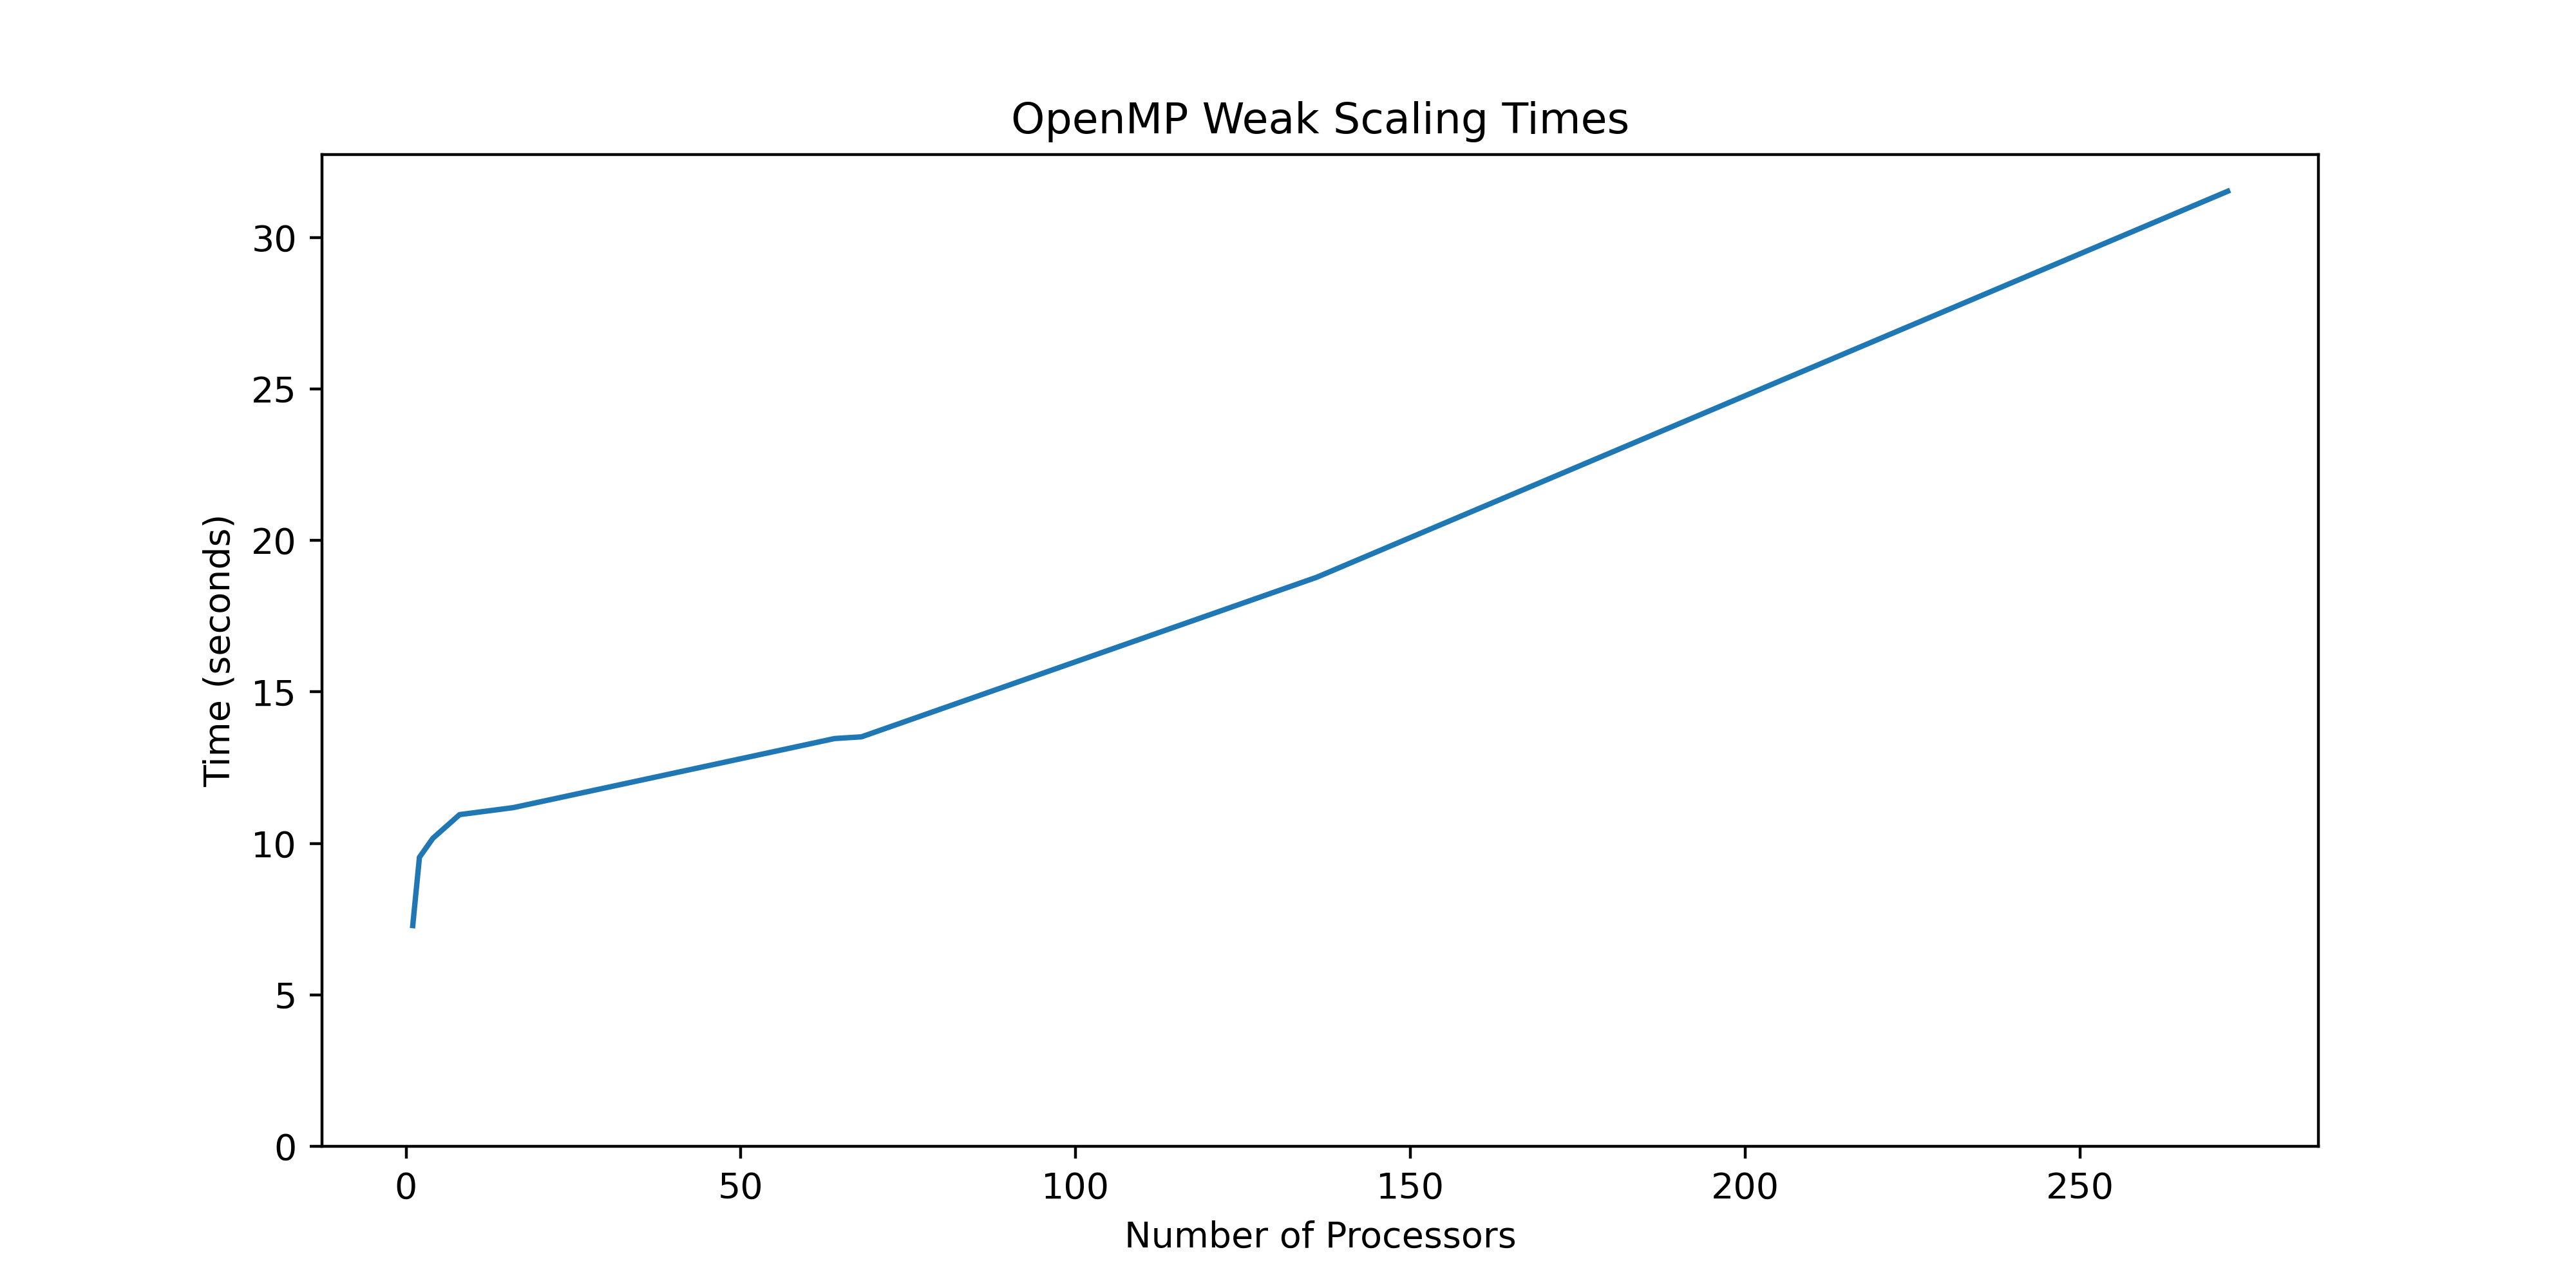
\includegraphics[width=6in]{figures/openmp_weak_scaling_times.png}
\caption{OpenMP Weak Scaling}
\label{fig:openmp-weak-scaling}
\end{figure}

Figure \ref{fig:openmp-weak-scaling} shows the weak scaling when scaled up to all 272 threads of the Intel KNL processor. We set the number of particles initially to 10000 and scale the the number of particles with number of threads or processors with $p$. We made sure that processors were evenly spread by setting the environment variable \verb|OMP_PLACES=cores| and \verb|OMP_PROC_BIND=spread|.

In an ideal weak scaling scenario, we would expect to see a horizontal line for a serial runtime of $O(n)$ complexity. But we see that as the work increases, the time also increases as well, indicating that there must some overhead. Because not all of the simulation is parallelizable, we are also facing Amdahl's (Heartbreaking) Law. We reach just over 30 seconds for a simulation on all 272 threads on the KNL processor. 

\begin{figure}[H]
\centering
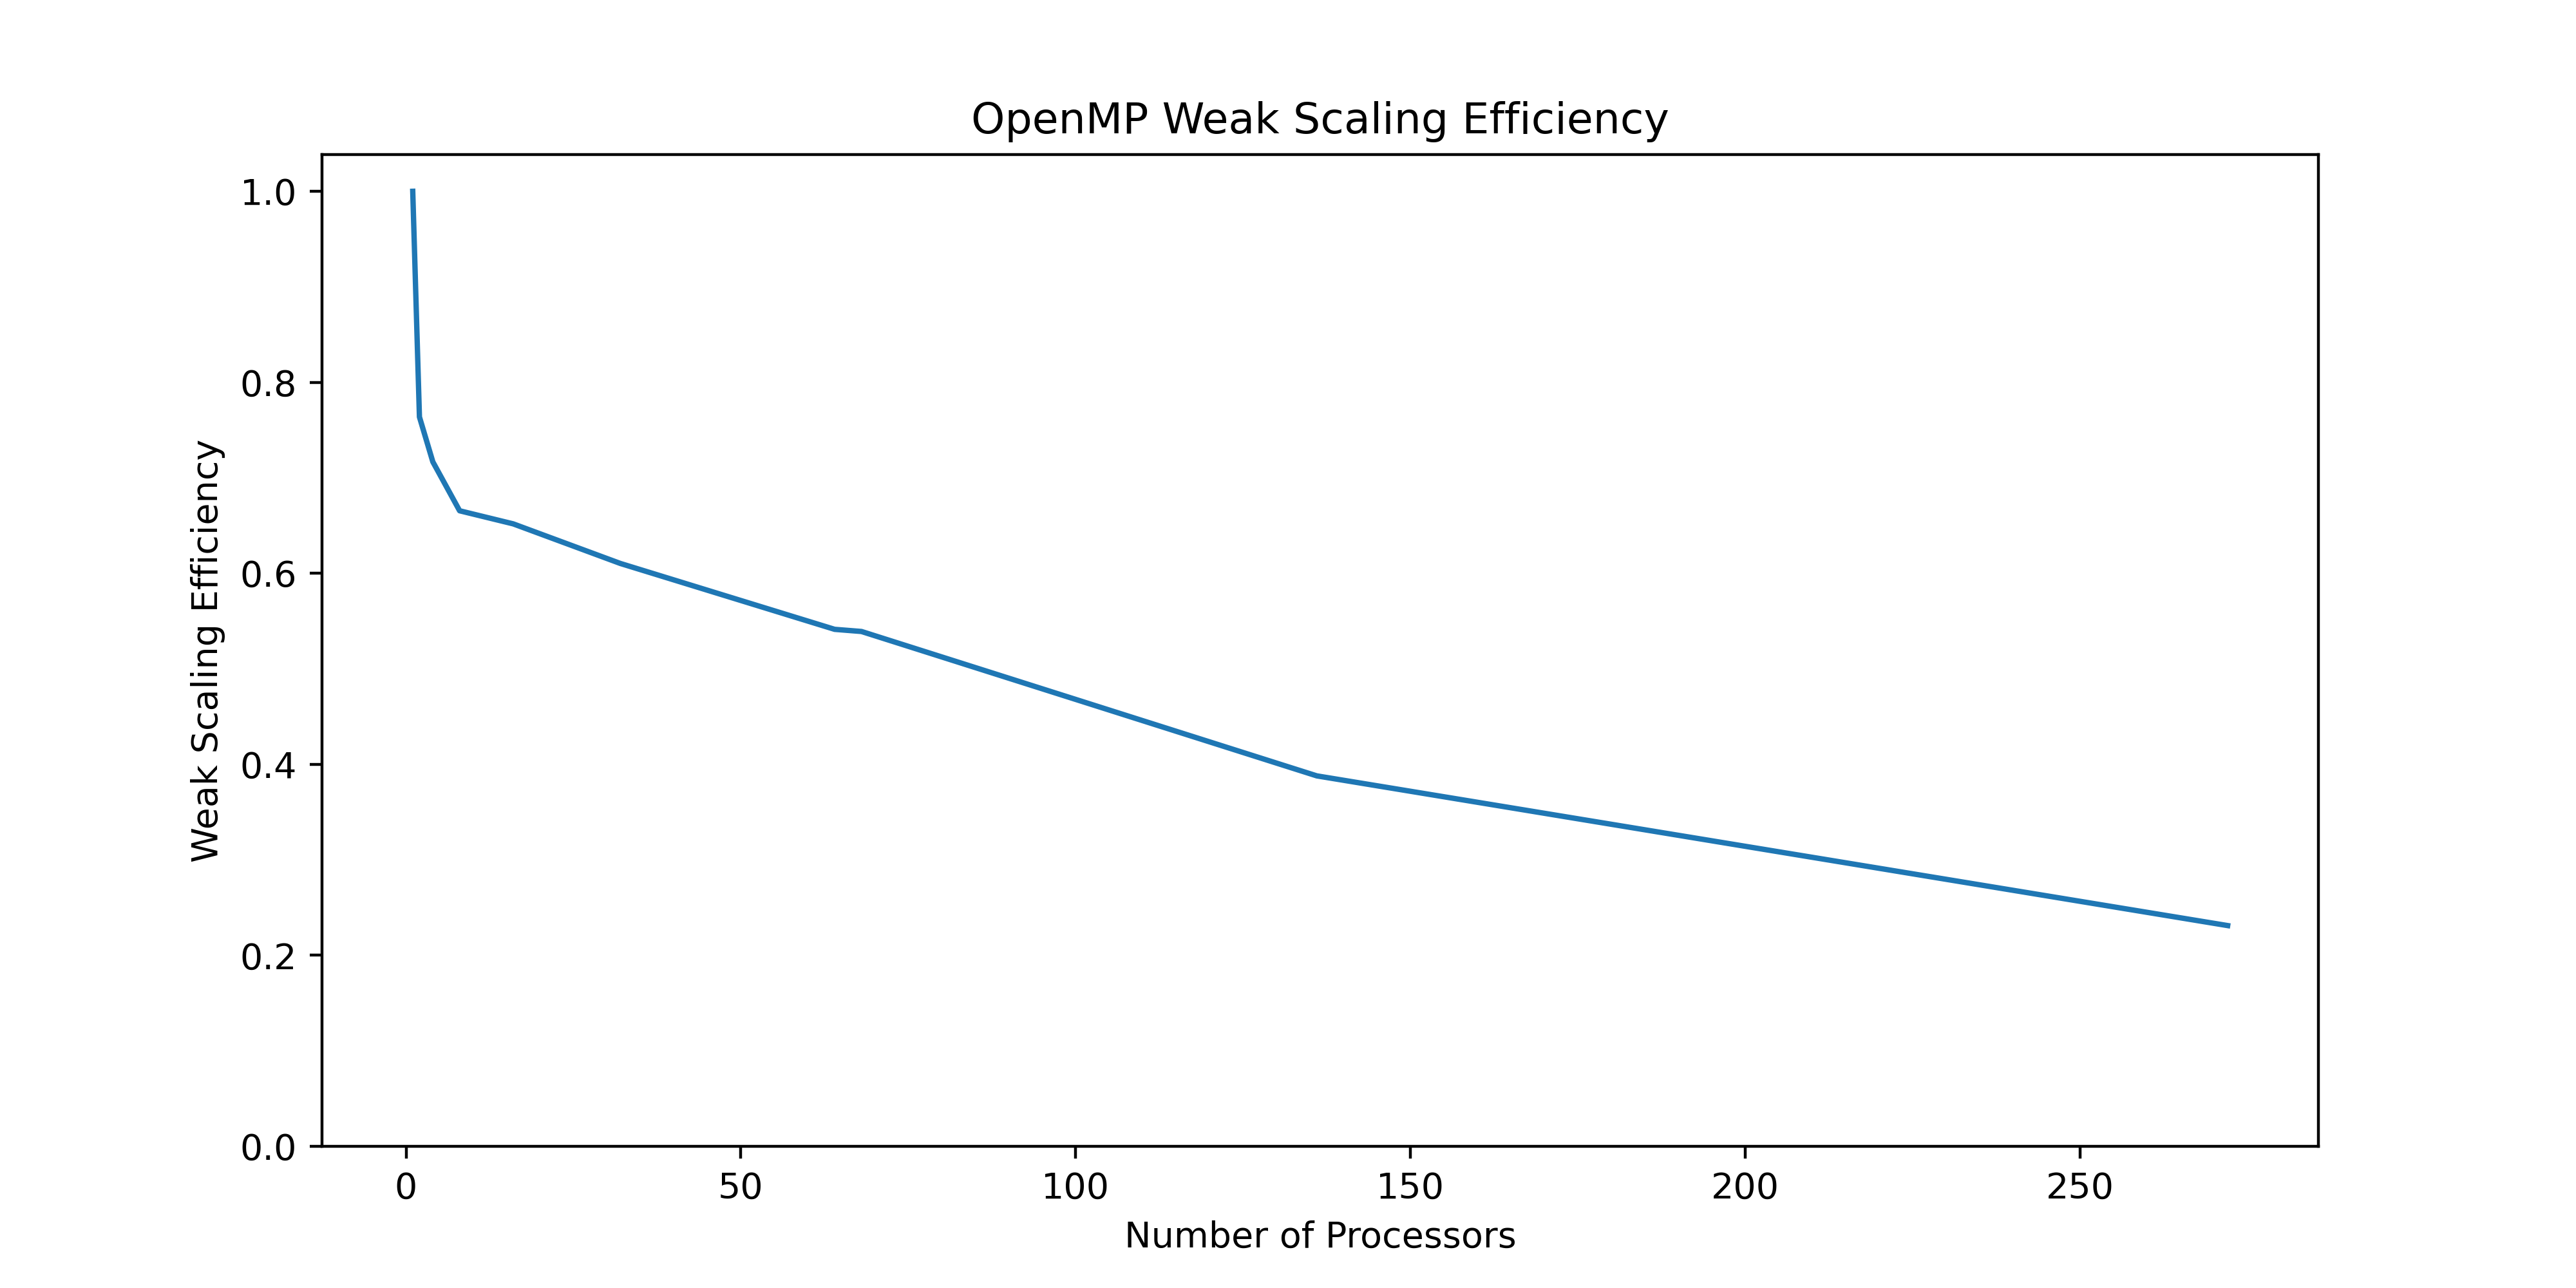
\includegraphics[width=6in]{figures/openmp_weak_scaling_efficiency.png}
\caption{OpenMP Weak Scaling Efficiency}
\label{fig:openmp-weak-scaling-efficiency}
\end{figure}

Figure \ref{fig:openmp-weak-scaling-efficiency} shows the weak scaling efficiency of our $n$-body simulation on OpenMP. We can see that our weak scaling efficiency is obviously highest at 1 processor. But it drastically decreases when we are at 2 processors down to 75\%. This large drop off may be due a large overhead of lock contention or any other synchronization overheads that wouldn't occur in a single threaded context. We see that is indeed the case in our analysis of performance breakdown later on.

We began to notice that utilizing all the 4-way hyperthreading on Intel KNL processor did not bring any significant speedups. This is mainly due to a core having only one ALU and 4 hyperthreads competing for resources. Thus, there is not much speedup since our simulation is arithmetically intensive. To accurately benchmark and analyze our performance, we tried again at a finer grain level by rerunning weak scaling from 1 to 68 cores. 

Figure \ref{fig:openmp-weak-scaling-fine} shows the weak scaling times, and we clearly see that it looks much better. Our performance looks more like a horizontal line and we are sustaining performance after 2 processes or OpenMP threads. We start at 7.34 seconds at 1 core and reach a maximum of 13.50 seconds at 68 cores. The jump to two processors causes time to increase to 9.61 seconds, and we gradually increase the number of work per processor as we scale the number of work with cores. 

\begin{figure}[H]
\centering
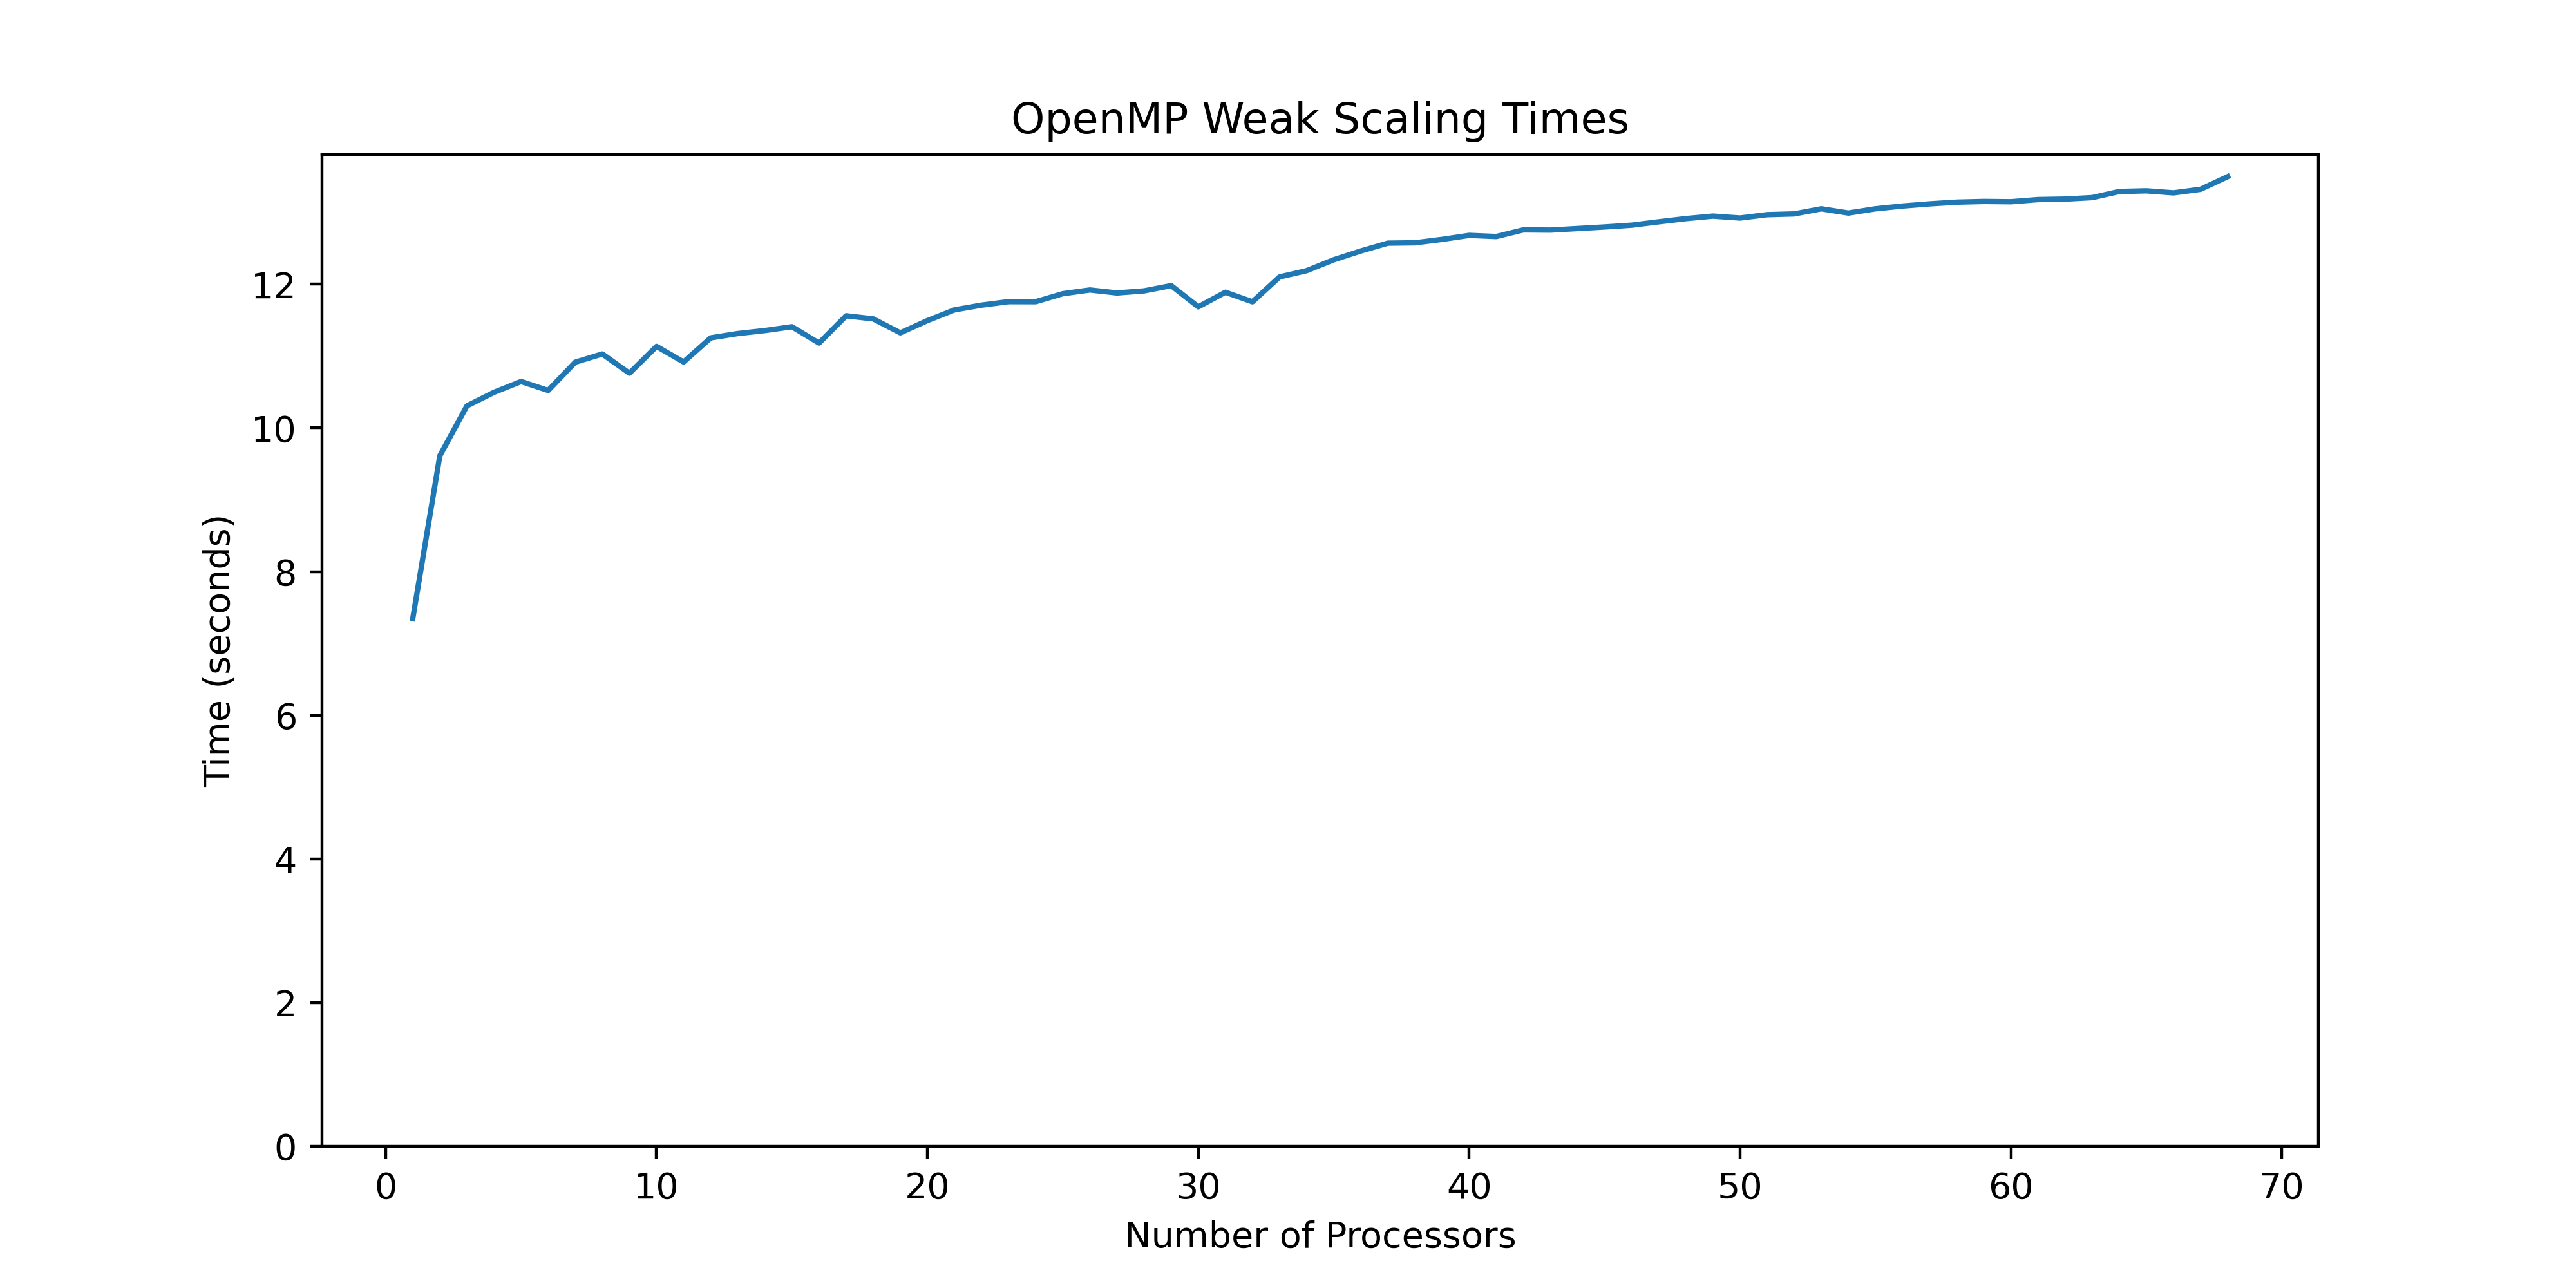
\includegraphics[width=6in]{figures/openmp_weak_scaling_times_fine.png}
\caption{OpenMP Weak Scaling Fine}
\label{fig:openmp-weak-scaling-fine}
\end{figure}

In Figure \ref{fig:openmp-weak-scaling-efficiency-fine}, we see the efficiency at a fine grain level. Again, we see that it is sustained around 60\%. Looking at how horizontal the line is compared to the previous results with all 272 threads, the efficiency is still bad. But how the scaling is sustained after the initial overhead, we see that these show some good scaling.

\begin{figure}[H]
\centering
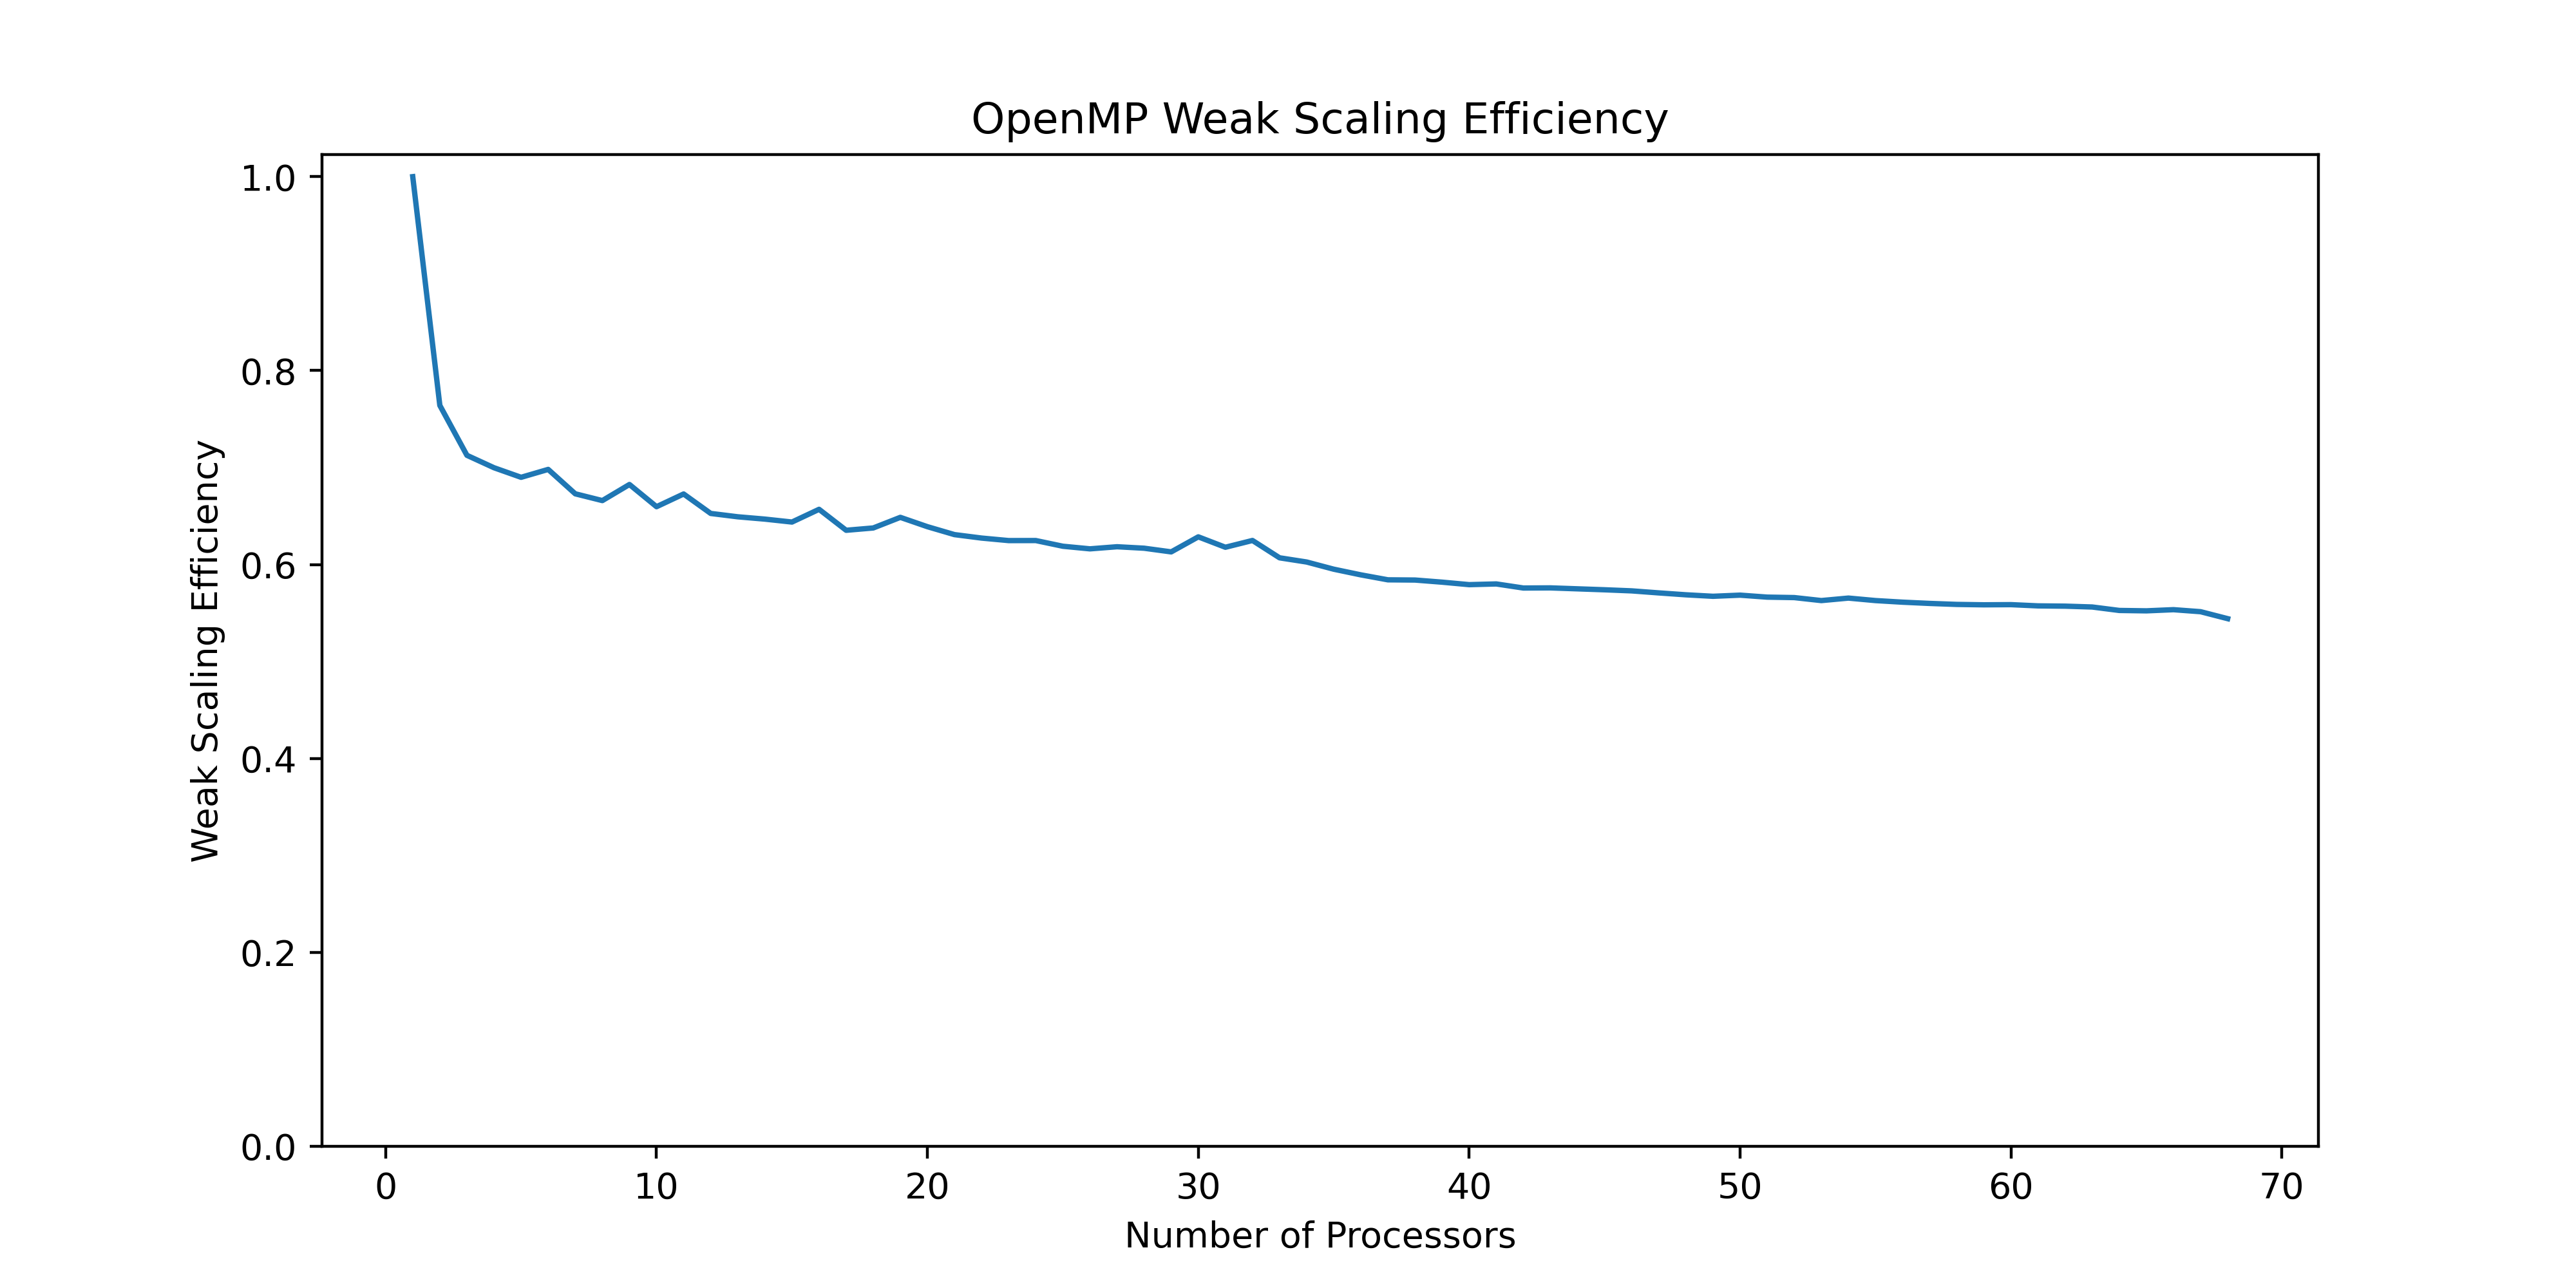
\includegraphics[width=6in]{figures/openmp_weak_scaling_efficiency_fine.png}
\caption{OpenMP Weak Scaling Efficiency Fine}
\label{fig:openmp-weak-scaling-efficiency-fine}
\end{figure}

\begin{figure}[H]
\centering
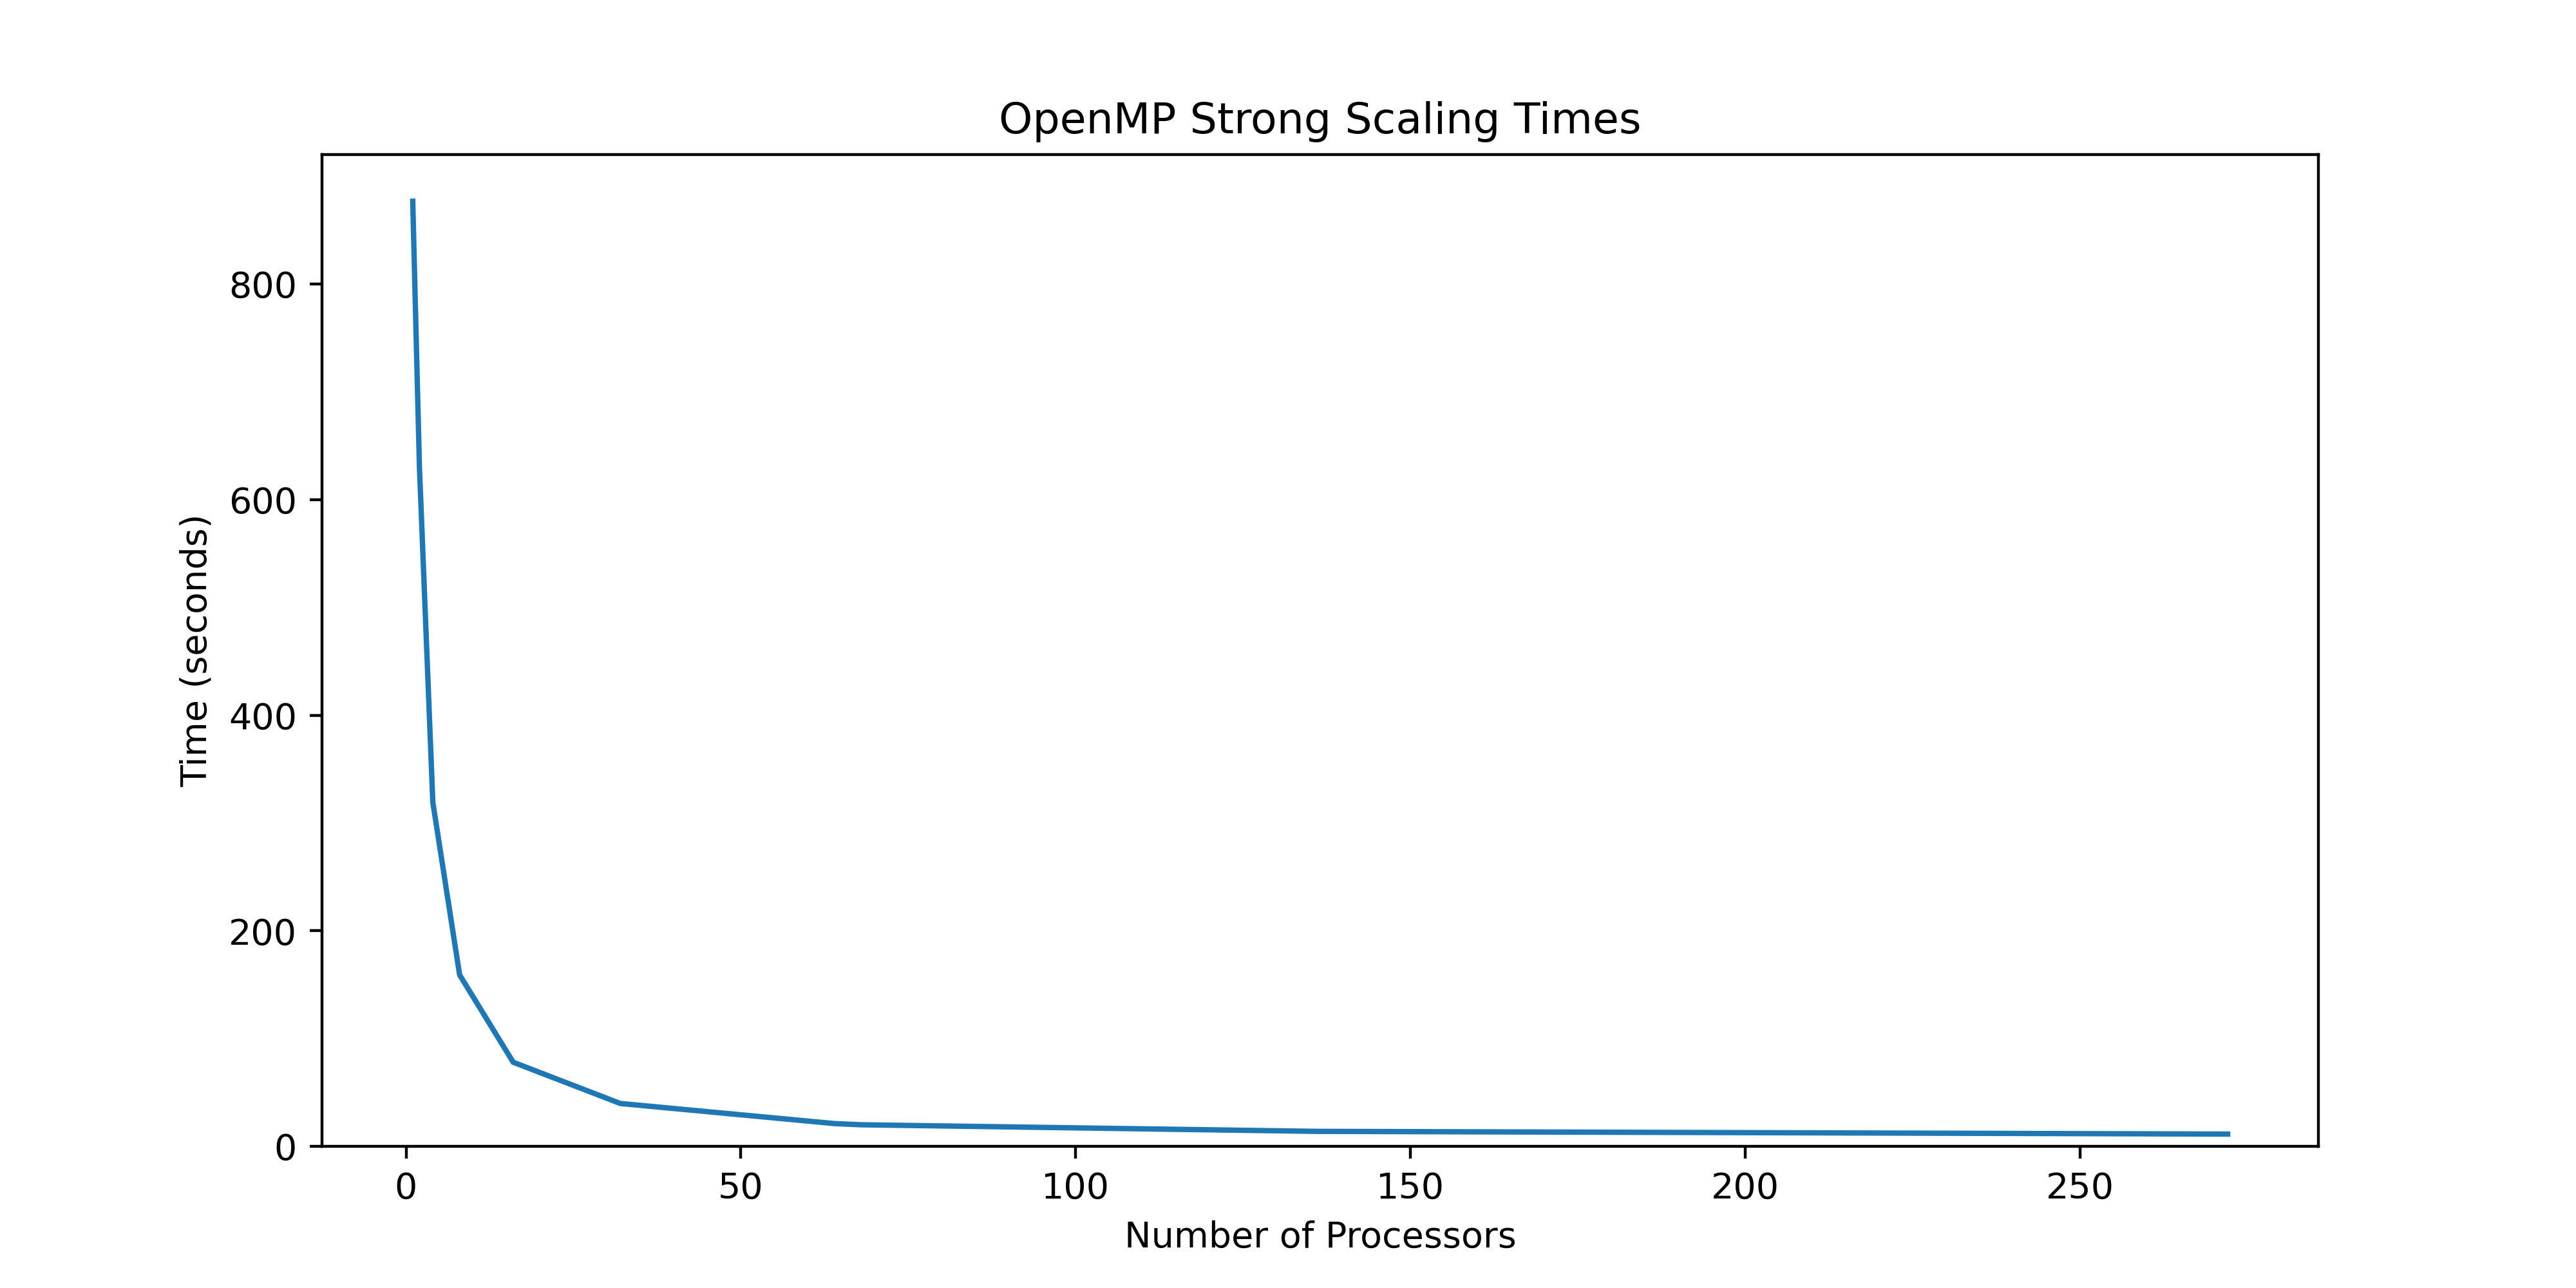
\includegraphics[width=6in]{figures/openmp_strong_scaling_times.png}
\caption{OpenMP Strong Scaling}
\label{fig:openmp-strong-scaling}
\end{figure}

Next we did experiments on strong scaling on 1000000 particles, and only varied the number of processors or OpenMP threads. Figure \ref{fig:openmp-strong-scaling} shows the strong scaling time. As expected, the time decreases as we increase the number of processors. We start from 876.91 seconds on one thread to 20.04 seconds to 272 threads, giving us a $43.7\times$ speedup. Although that is not $272\times$ speedup, it is still pretty substantial speedup.

\begin{figure}[H]
\centering
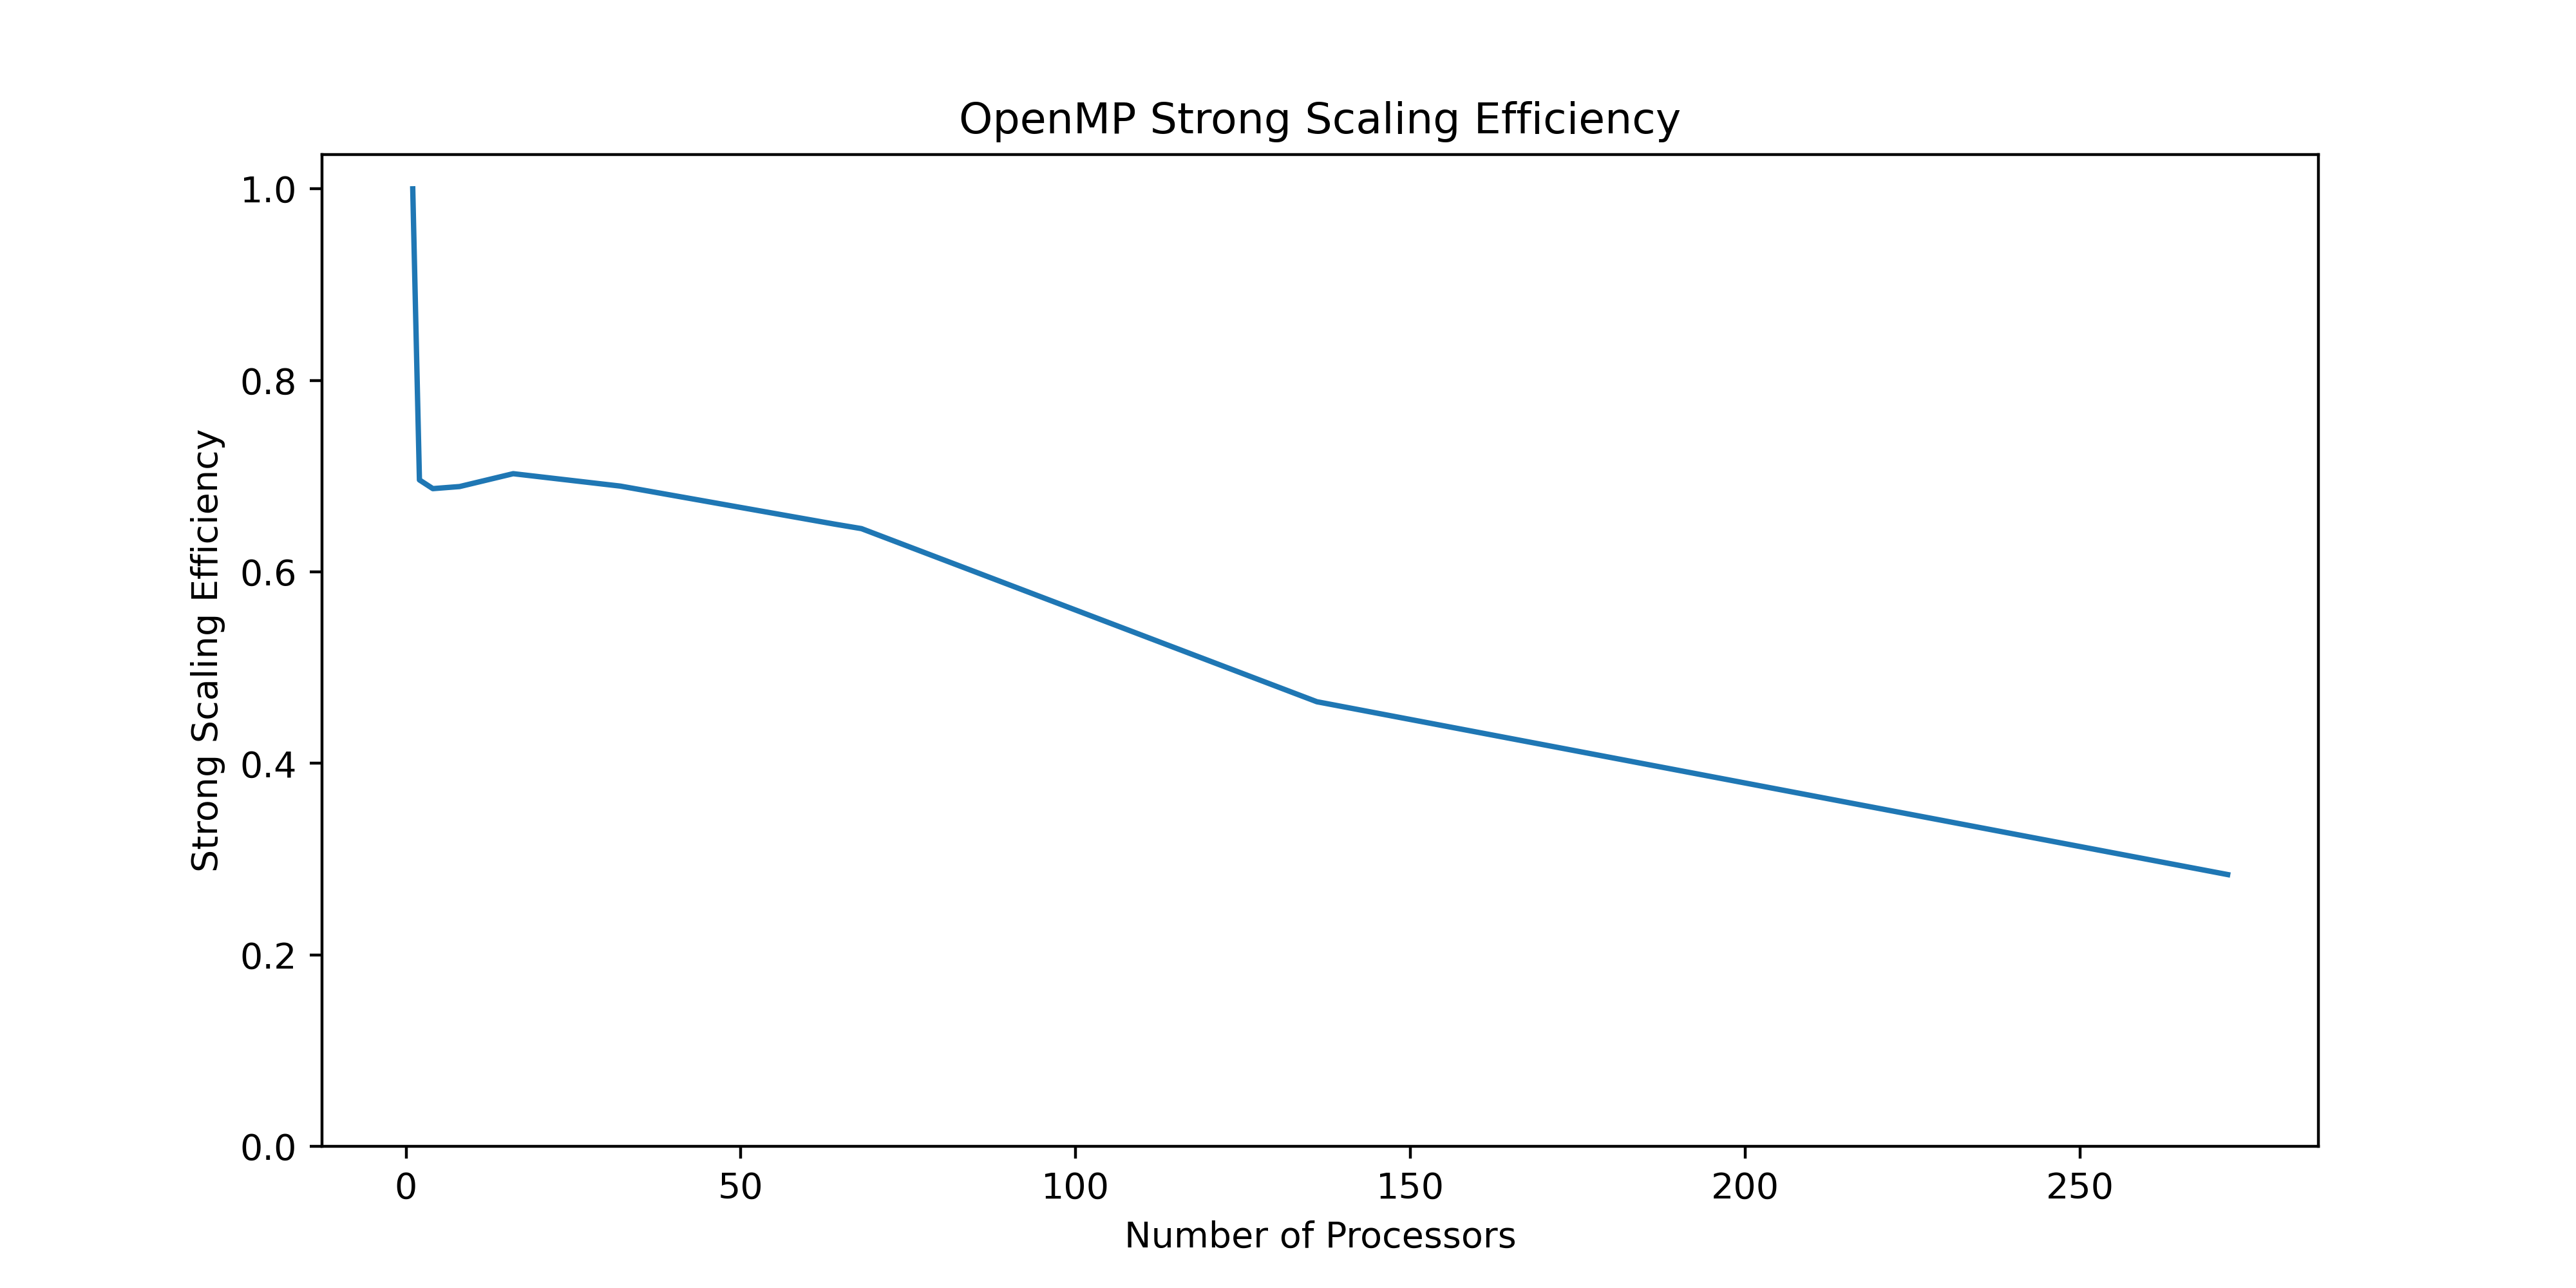
\includegraphics[width=6in]{figures/openmp_strong_scaling_efficiency.png}
\caption{OpenMP Strong Scaling}
\label{fig:openmp-strong-scaling-efficiency}
\end{figure}

To see this better, we observe the strong scaling efficiency shown in Figure \ref{fig:openmp-strong-scaling-efficiency}. We see that the efficiency drops to around 71.3\% at 2 threads or processors. When scaled up to all 272 threads, we get a disappointing efficiency of 28.4\%. Again, we have the same suspicions from weak scaling, where our simulation becomes not as efficient with the utilization of hyperthreads.

\begin{figure}[H]
\centering
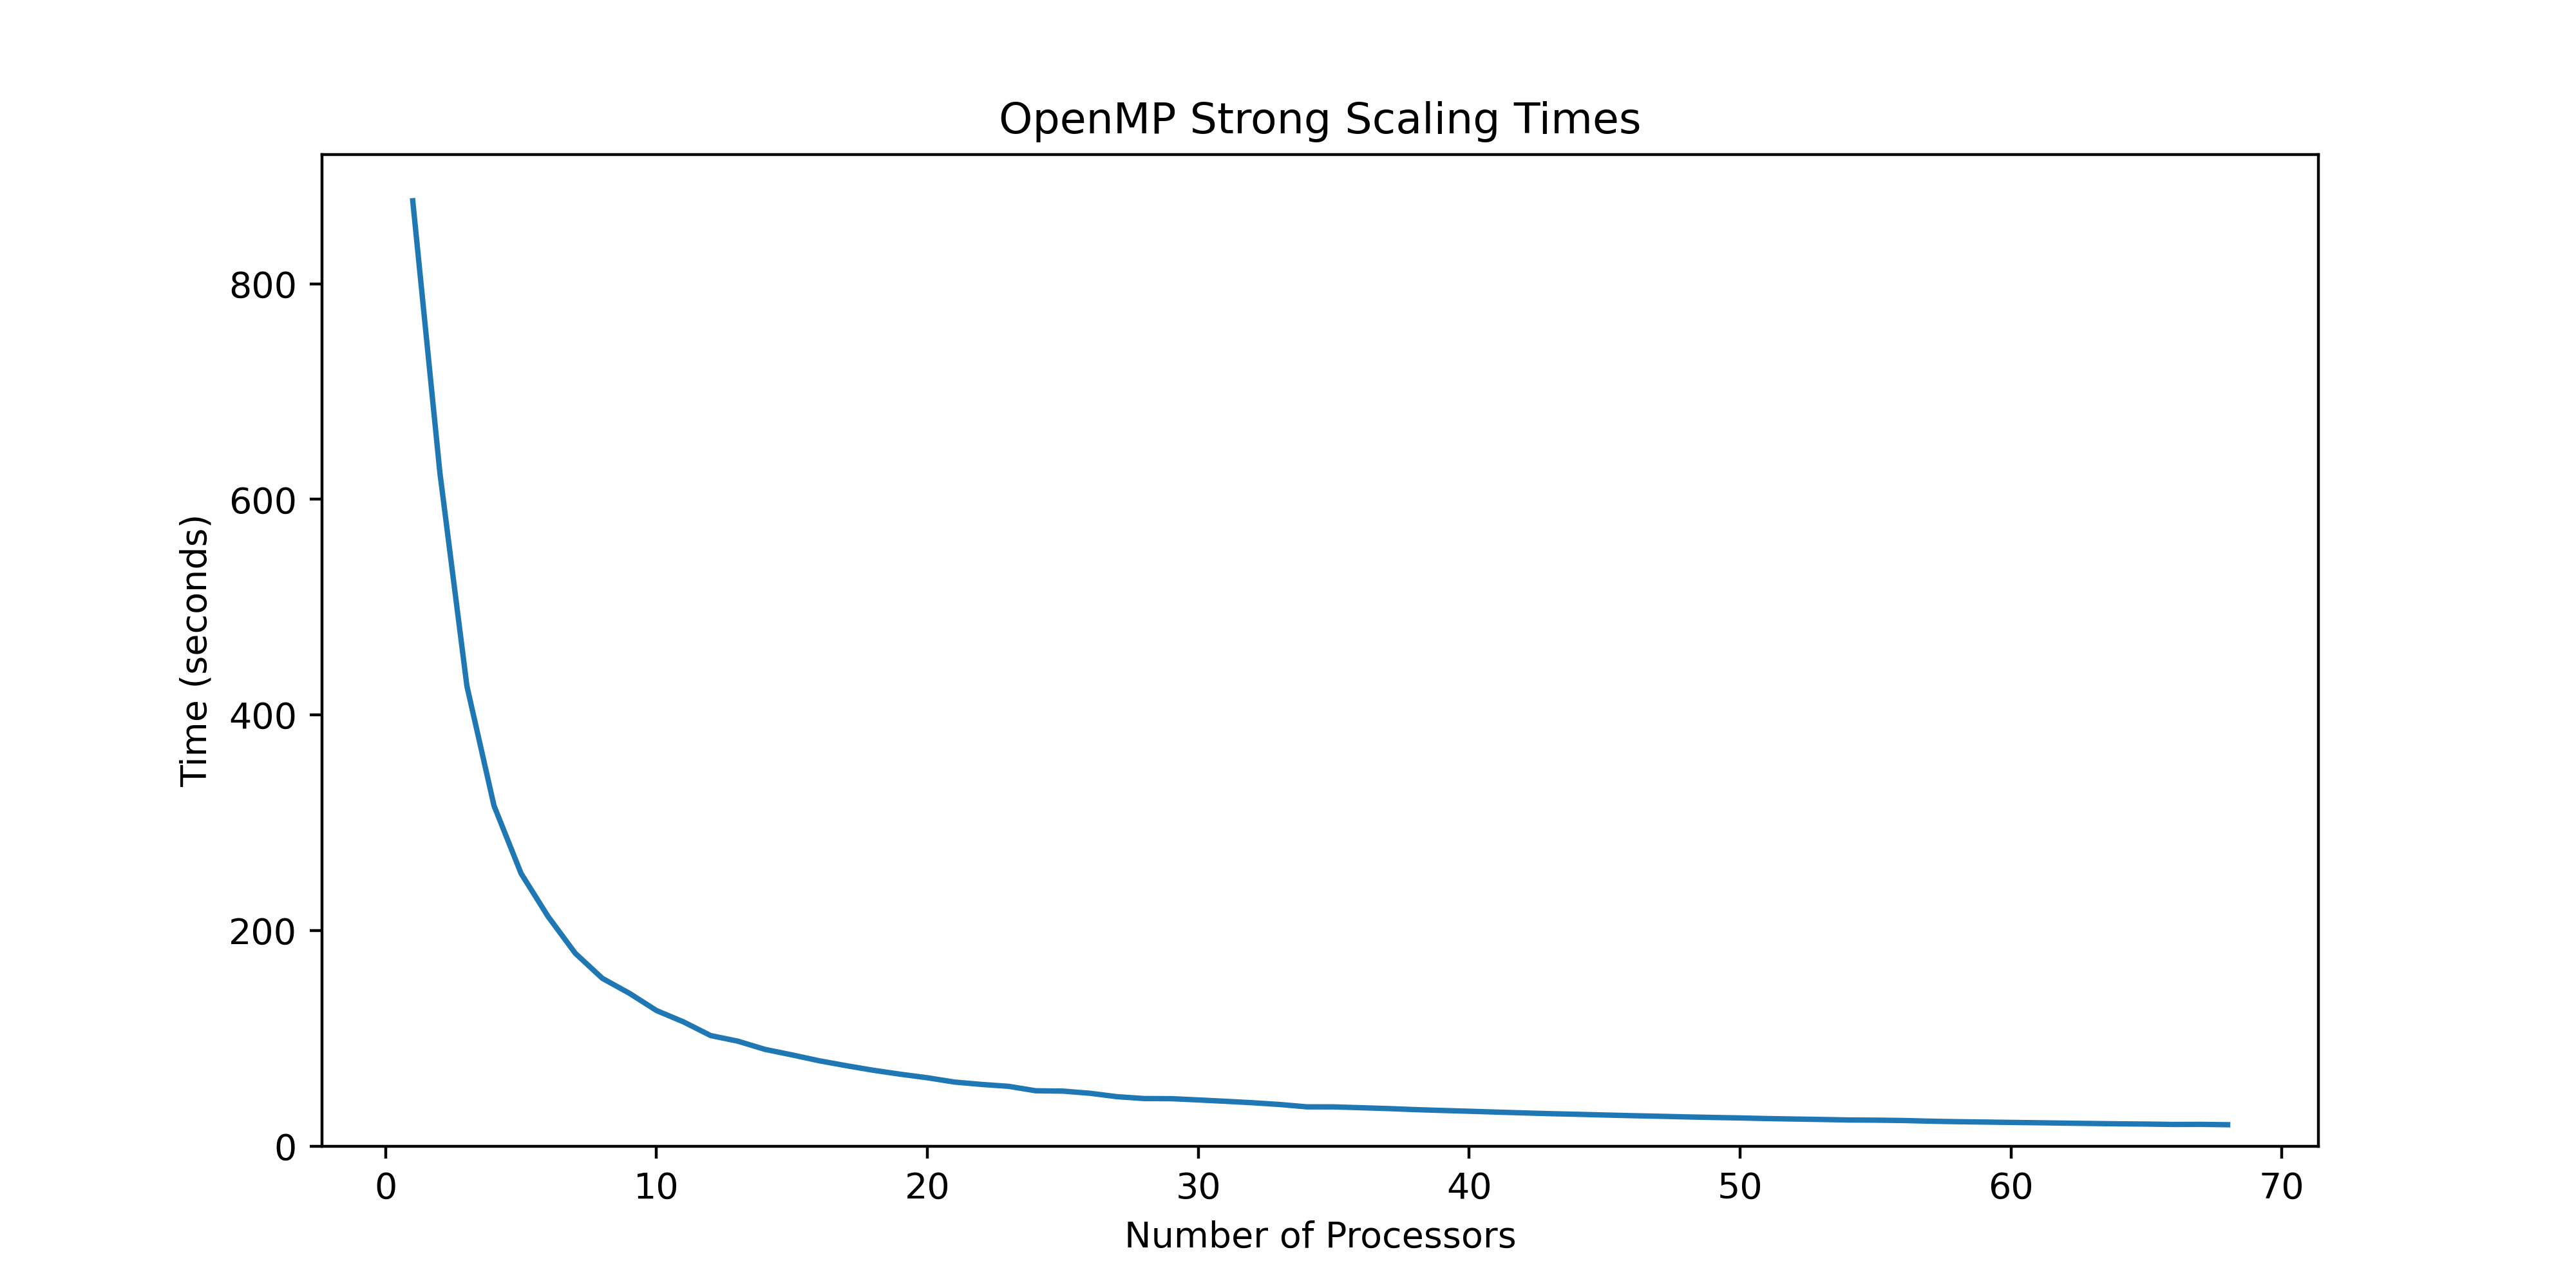
\includegraphics[width=6in]{figures/openmp_strong_scaling_times_fine.png}
\caption{OpenMP Strong Scaling Fine}
\label{fig:openmp-strong-scaling-fine}
\end{figure}

Figure \ref{fig:openmp-strong-scaling-fine} shows the strong scaling at a fine grain level up to only 68 cores/threads. To see the results better, Figure \ref{fig:openmp-strong-scaling-efficiency-fine} shows the strong scaling efficiency.

\begin{figure}[H]
\centering
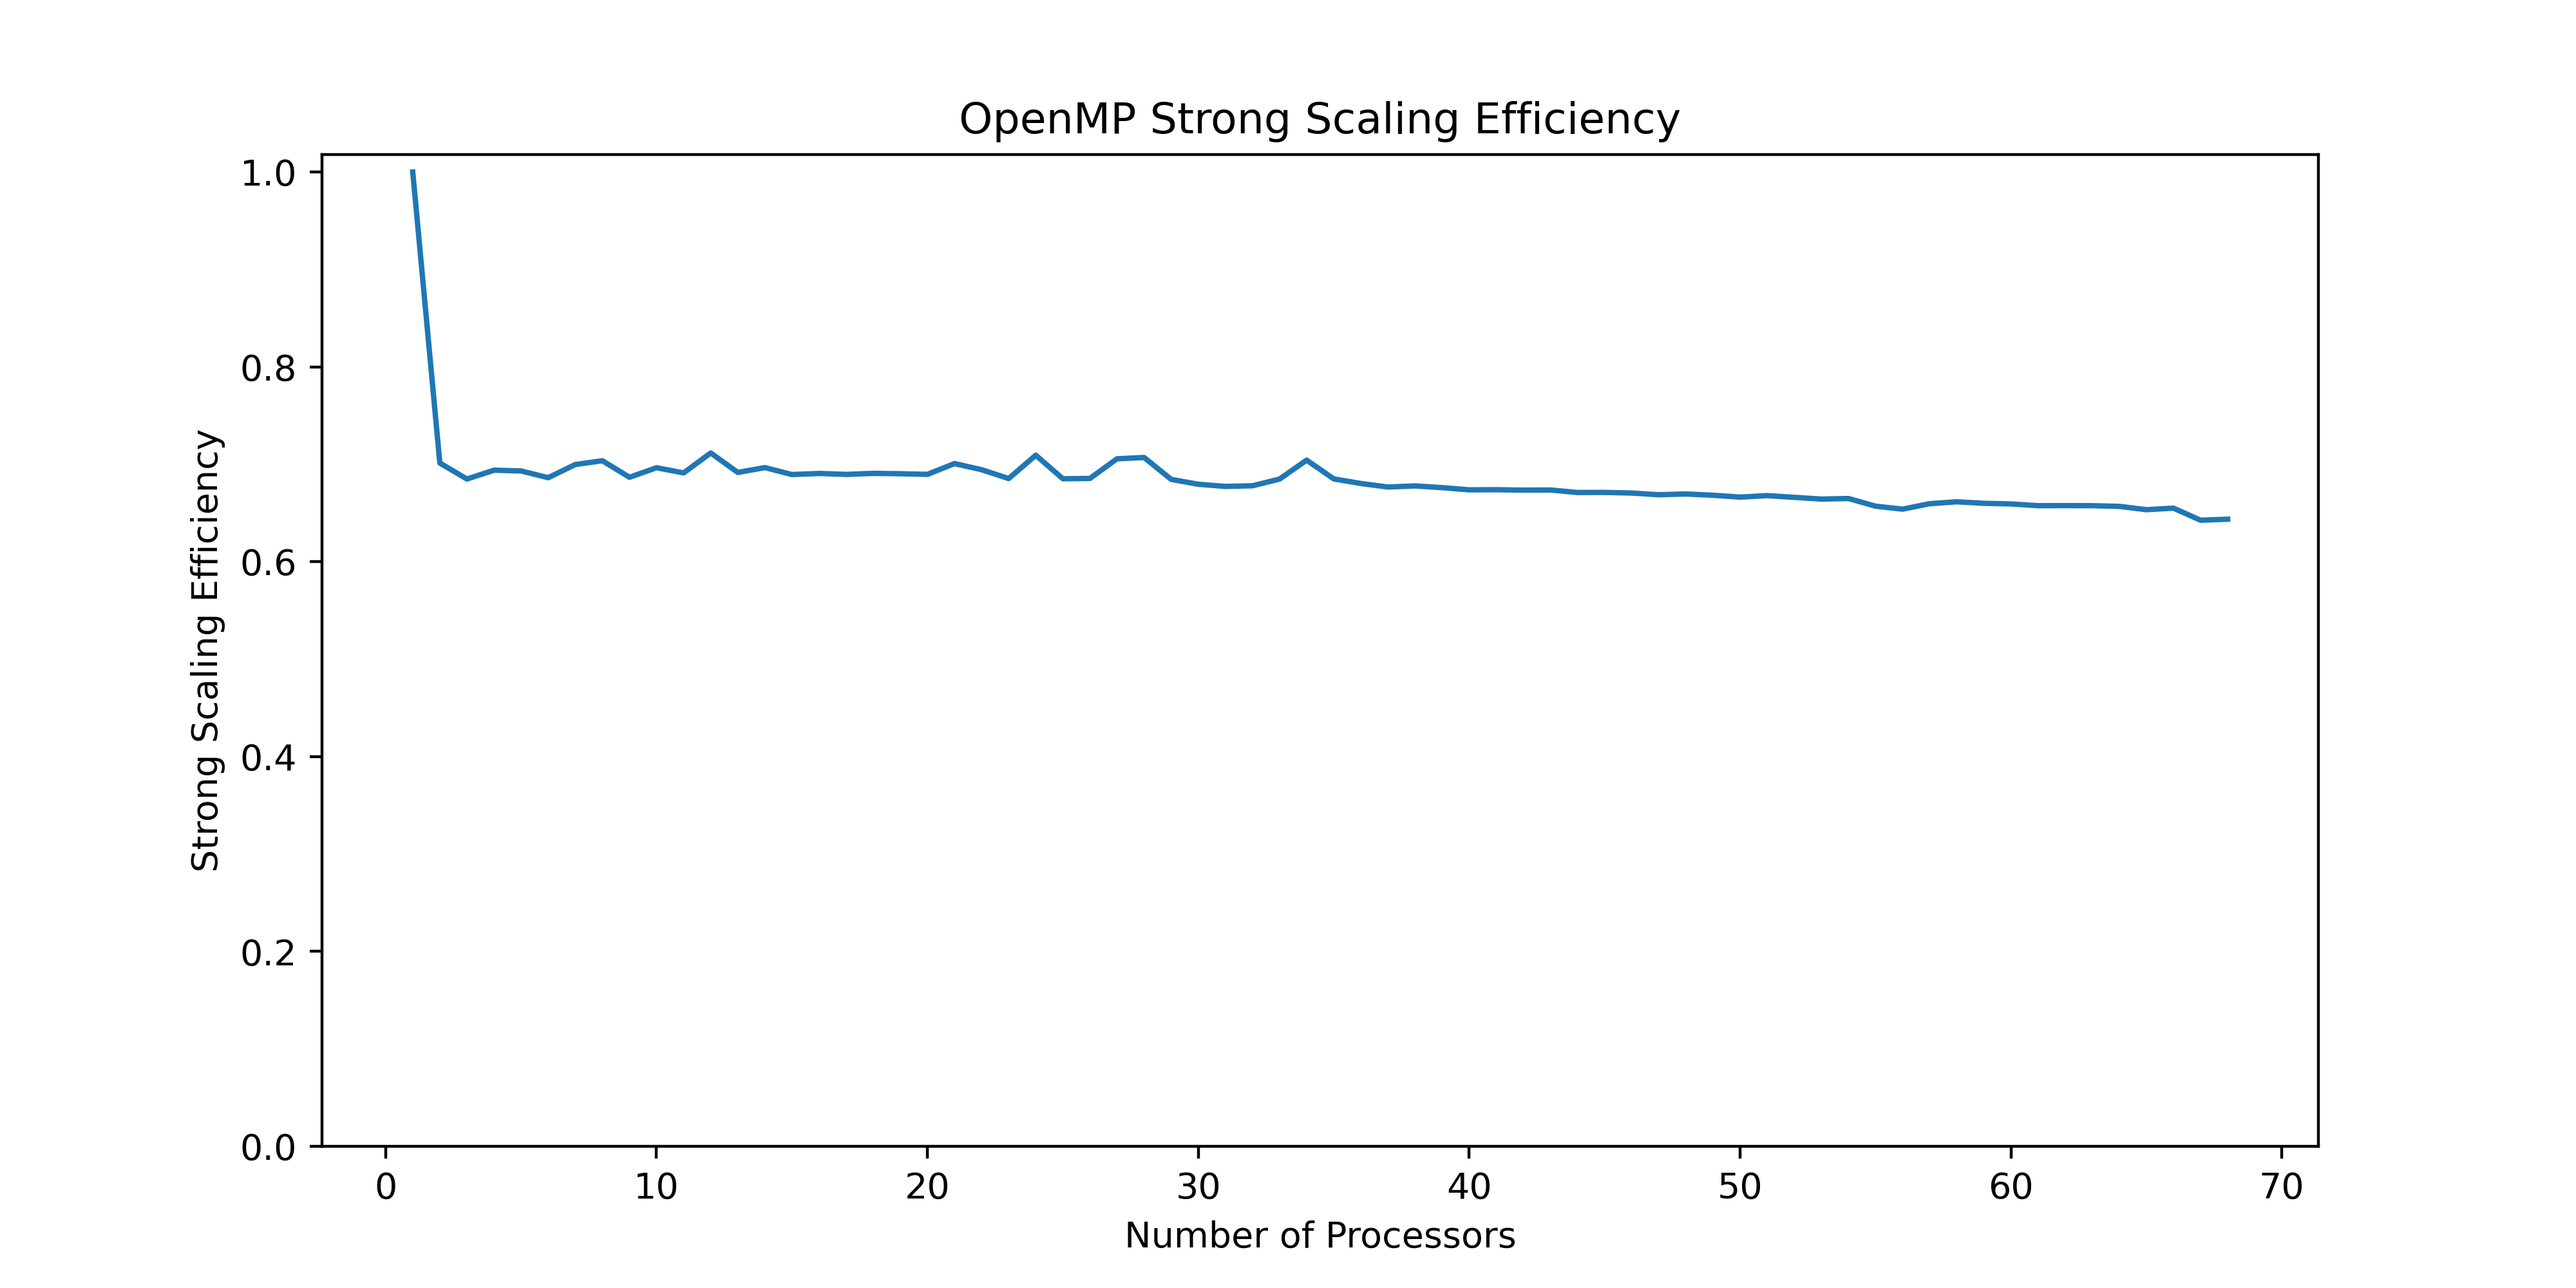
\includegraphics[width=6in]{figures/openmp_strong_scaling_efficiency_fine.png}
\caption{OpenMP Strong Scaling Efficiency Fine}
\label{fig:openmp-strong-scaling-efficiency-fine}
\end{figure}

The results look much better when looking at the efficiency, where the efficiency is sustained after 2 processors. At 2 processors or OpenMP threads, we have a strong scaling efficiency of 70.1\%. And that is slowly decreased to 64.4\% at 68 threads. Again, we see similar trends from weak scaling, where there is around 30\% overhead lost when scaling up to two threads. If we could've done this any better, we would've changed how to optimize the serial code to be more parallelizable to avoid these potential issues arised from lock contention.

\begin{figure}[H]
\centering
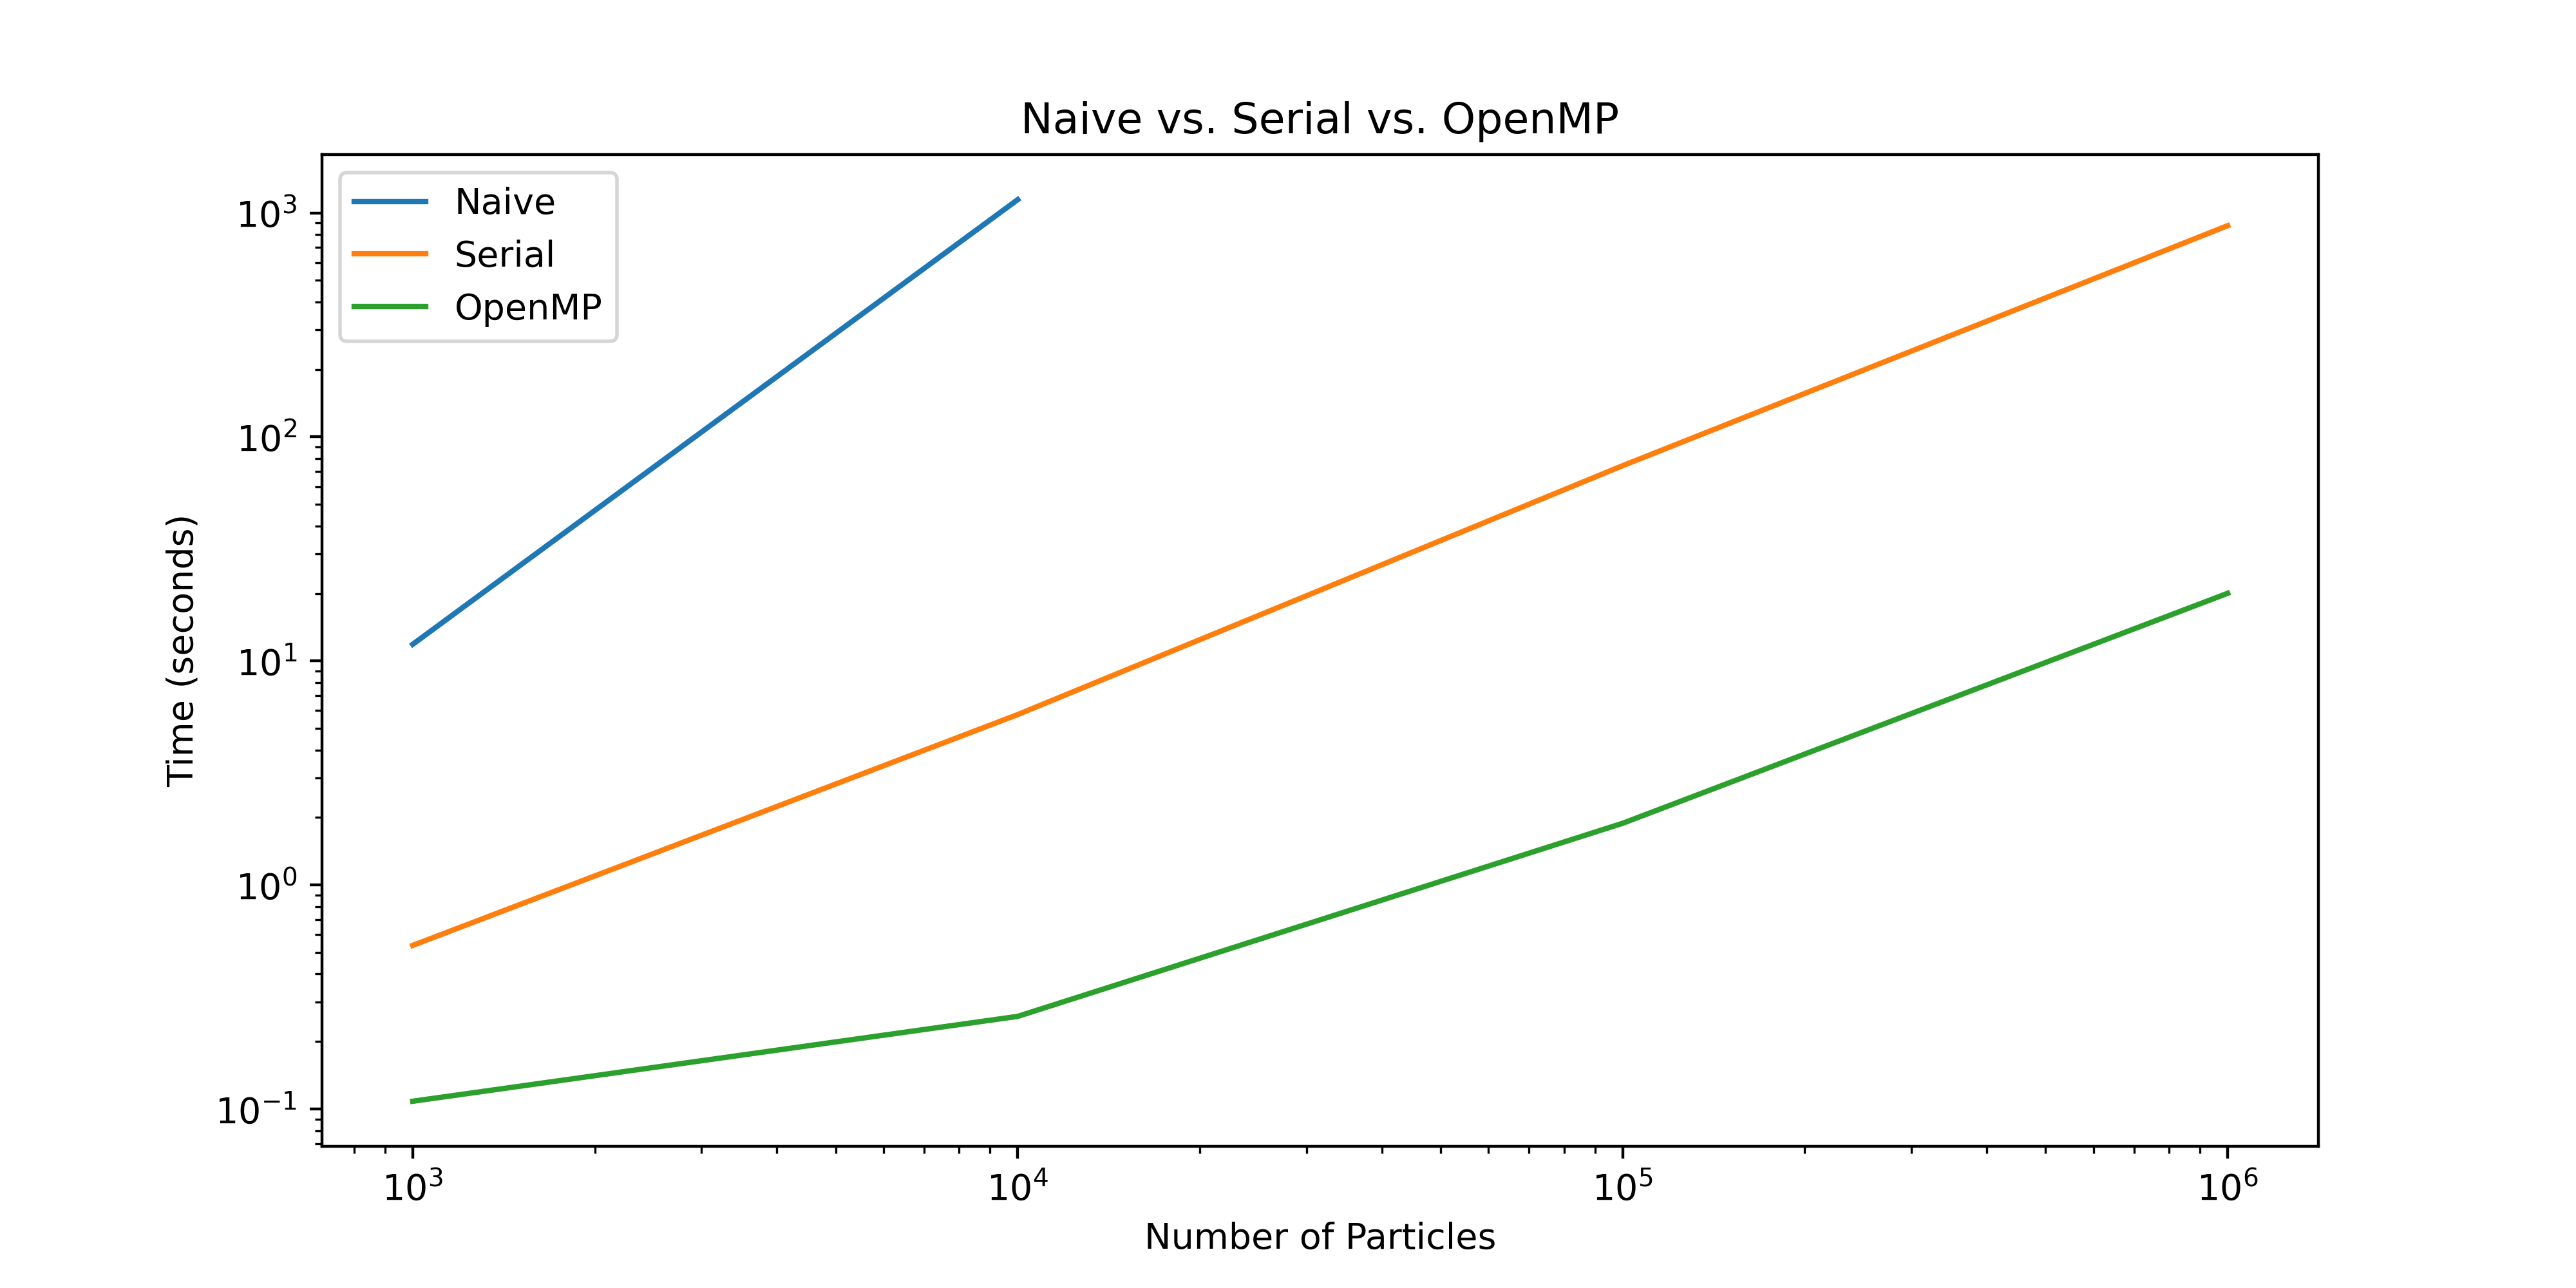
\includegraphics[width=6in]{figures/openmp_compared.png}
\caption{Naive vs. Serial vs. OpenMP}
\label{fig:openmp-compared}
\end{figure}

Figure \ref{fig:openmp-compared} compares all of the implementations on a log-log scale. We could not comprehensively collect results for the naive runtimes, since it would run too long, but we see that our serial $O(n)$ implemntations drastically speed it up and our OpenMP implementation accelerates and scales the performance even further.

\subsection{Performance Breakdown}
For performance breakdown, we profiled with ARM MAP. We first profiled our particle simulation on OpenMP with 1 million particles in order to collect enough samples for the trace.

\begin{figure}[H]
\centering
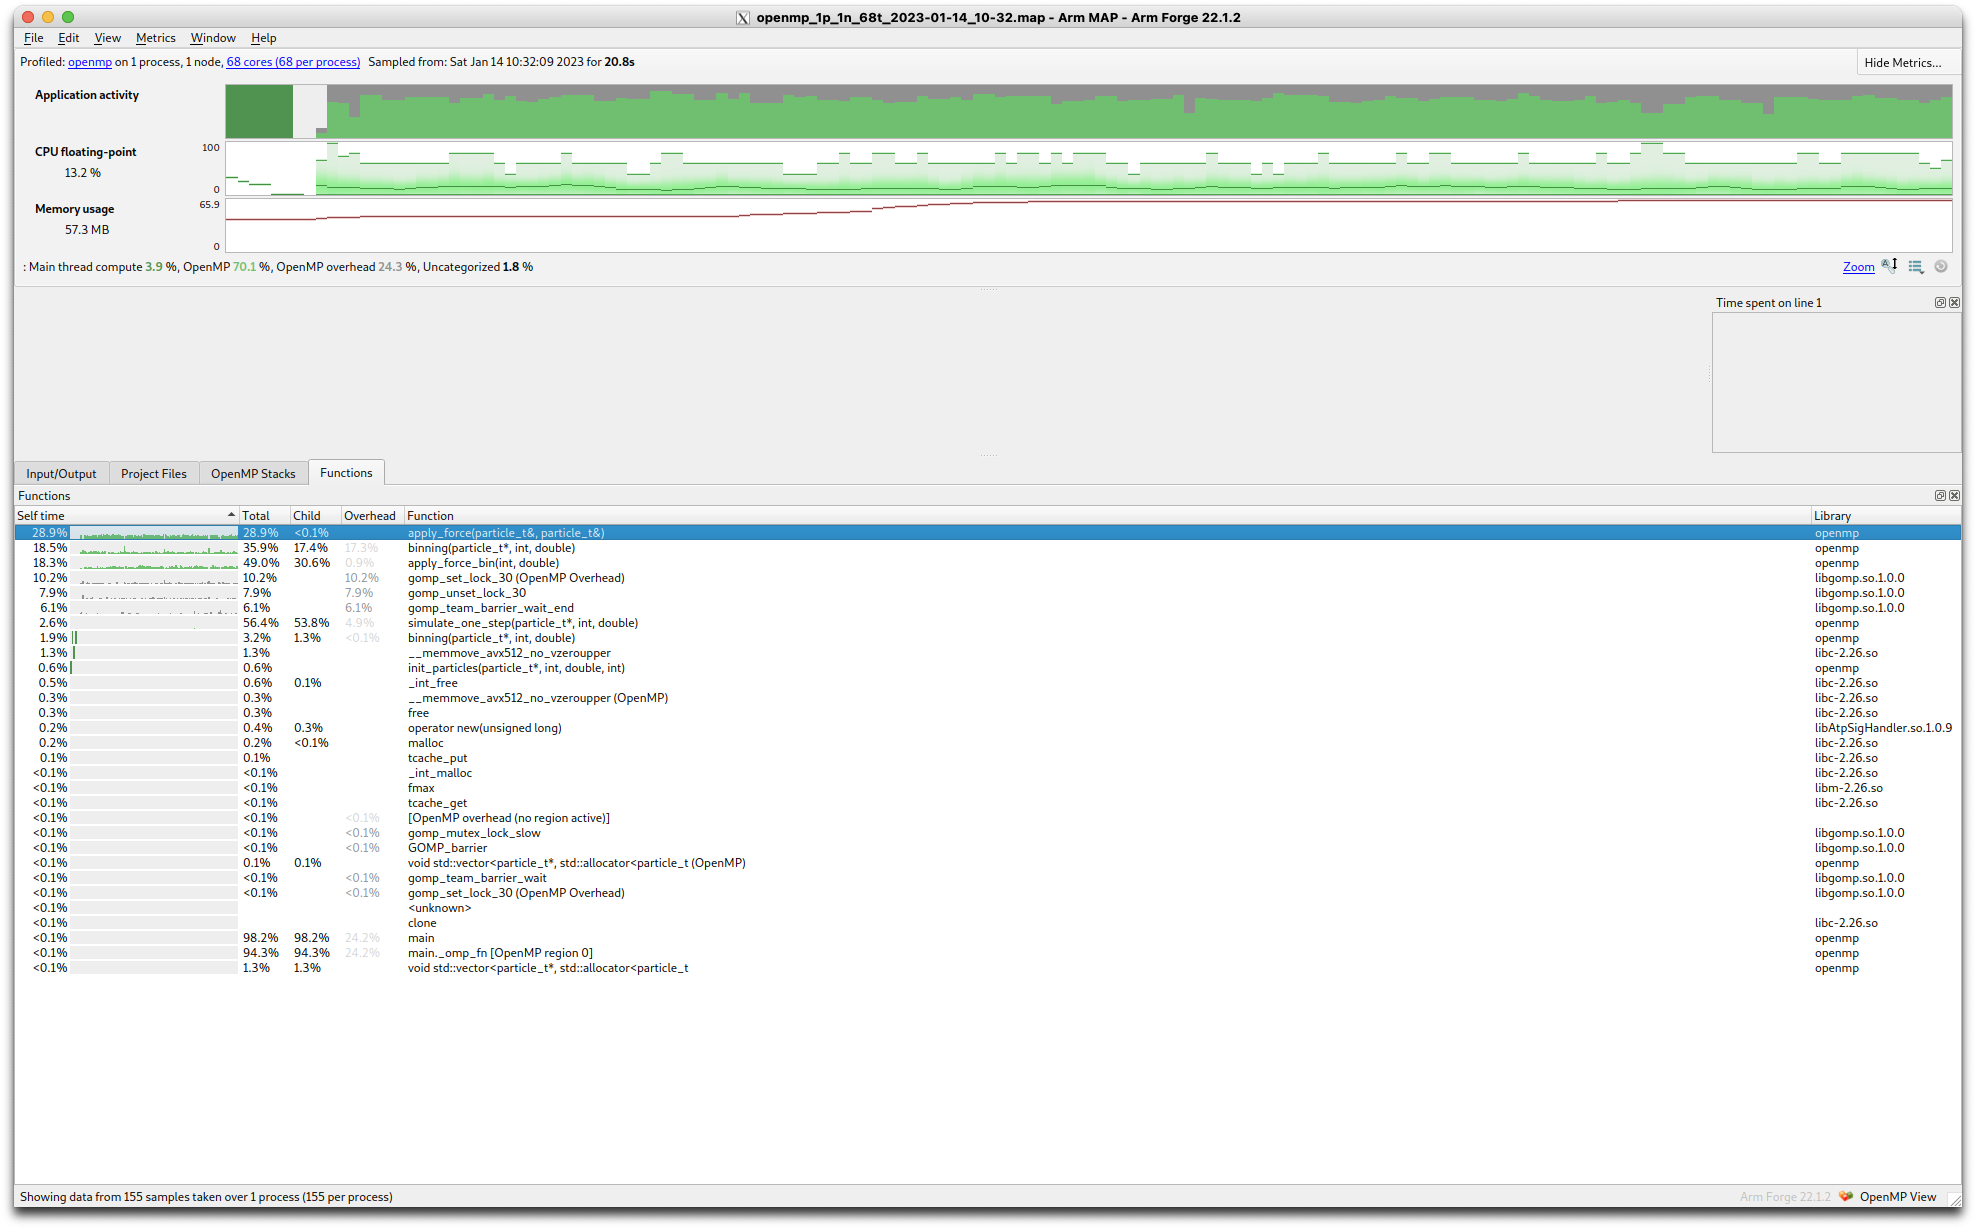
\includegraphics[width=6in]{figures/openmp-profile.png}
\caption{ARM MAP Profile Trace}
\label{fig:openmp-profile-trace}
\end{figure}

The ARM MAP tool was very simple and intuitive to use, and it gave us some clear insights about our performance and bottlenecks. Figure \ref{fig:openmp-profile-trace} shows a sample trace from a simulation of 1 million particles on 68 cores. We see that 3.9\% of our code was spent on the main thread, and 70.1\% of it was spent in OpenMP. There is 24.3\% spent in overhead of OpenMP, which is the initialization of OpenMP threads and any synchronization primitives. 1.8\% of the runtime was uncategorized. Considering that there is 30\% of non-parallelized code, this looked pretty good. And it also empirically supports our previous claim that not all of the code was parallizable. Thus, our huge dropoff in performance once we started scaling to two processors for both weak and strong scaling can be explained.

For a better understanding of how the compute and synchronization time is spent, we profiled simulations on 100000 particles on $p = {1, 2, 4, 8, 16, 32, 64, 68}$ processors. Figure \ref{fig:openmp-profile} shows the breakdown.

\begin{figure}[H]
\centering
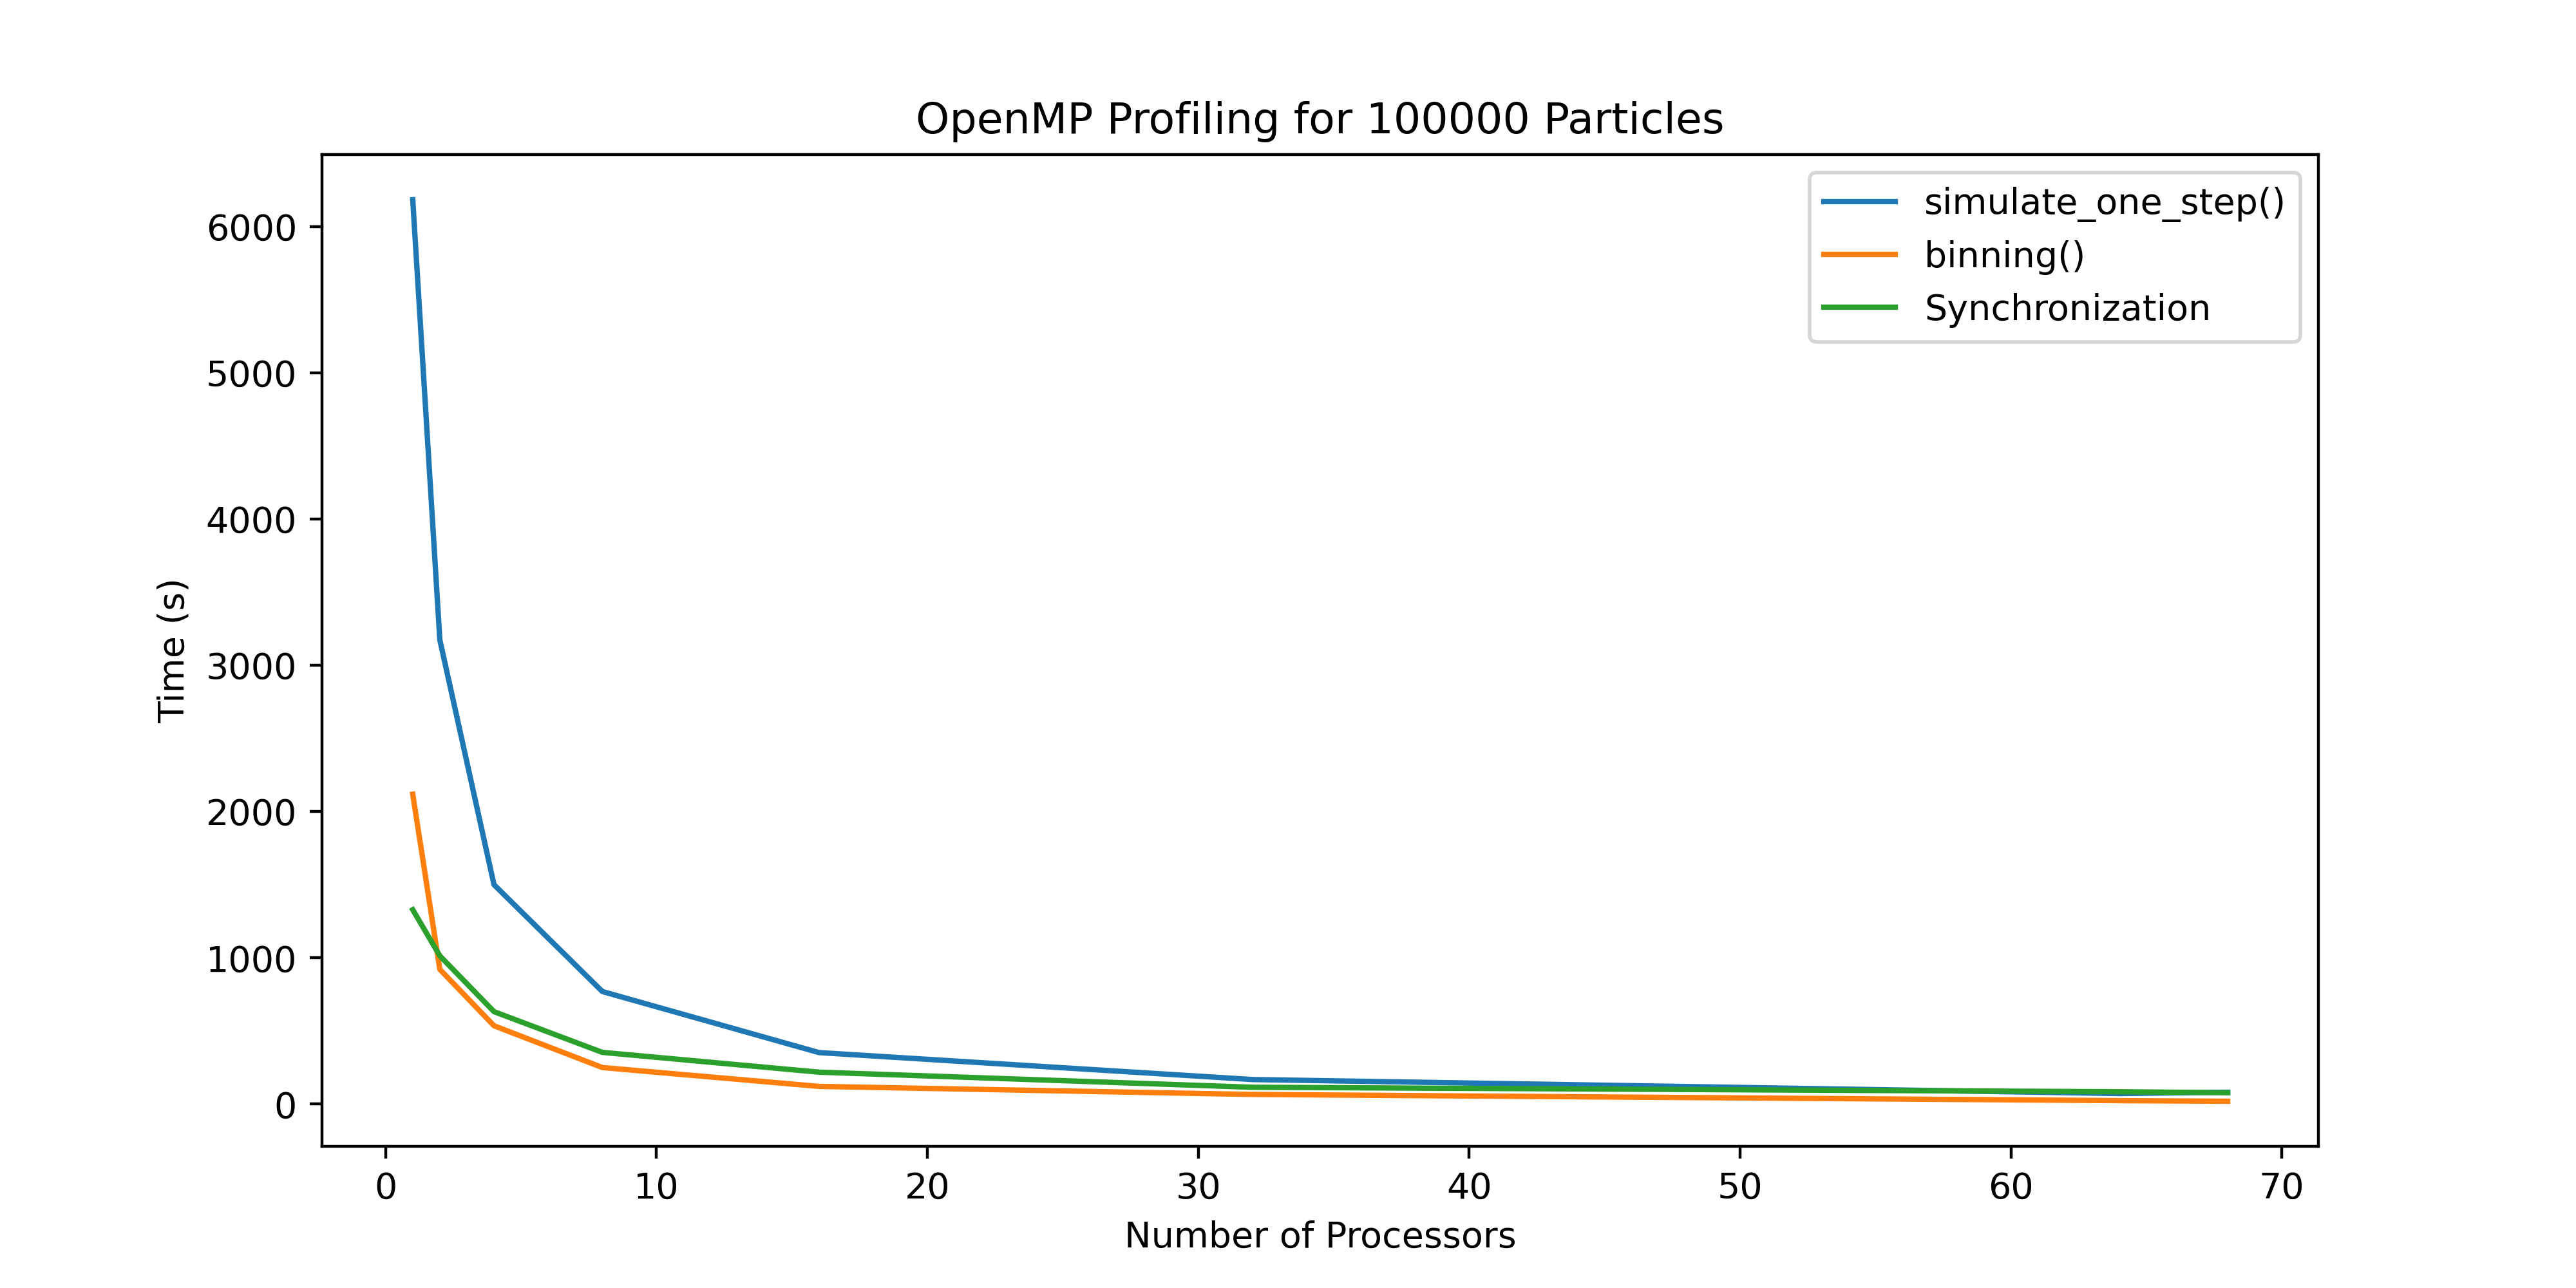
\includegraphics[width=6in]{figures/openmp_profiling.png}
\caption{OpenMP Performance Breakdown}
\label{fig:openmp-profile}
\end{figure}

Figure \ref{fig:openmp-profile-stacked} shows the breakdown stacked.

\begin{figure}[H]
\centering
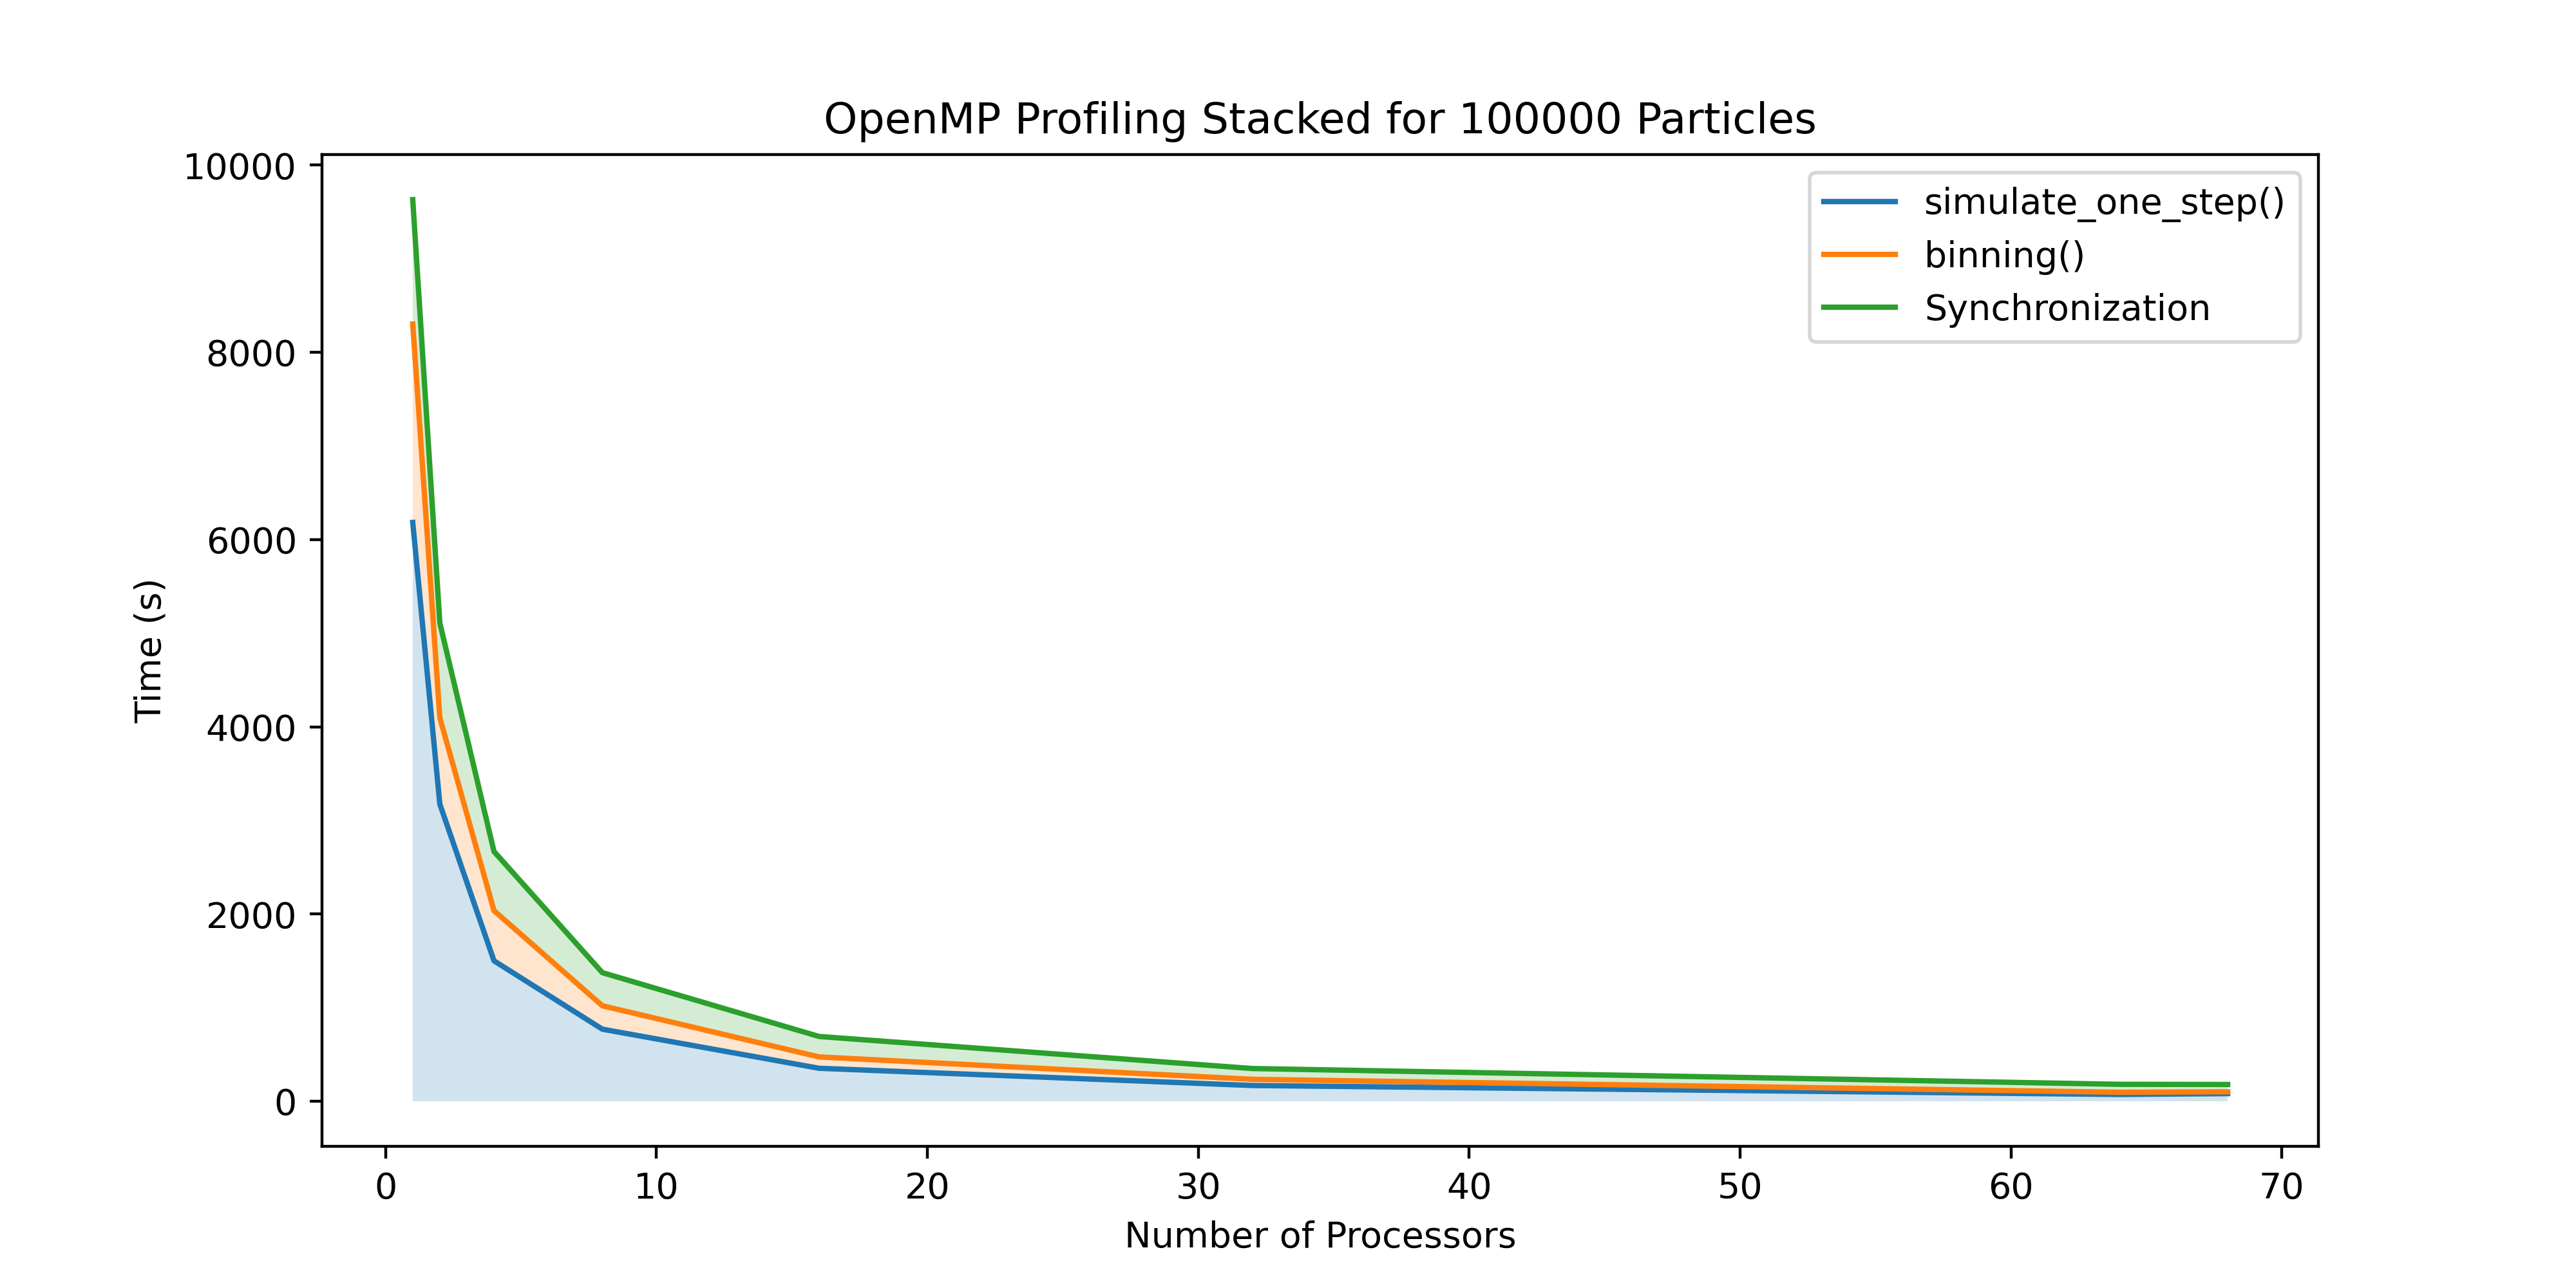
\includegraphics[width=6in]{figures/openmp_profiling_stacked.png}
\caption{OpenMP Performance Breakdown Stacked}
\label{fig:openmp-profile-stacked}
\end{figure}

Lastly, Figure \ref{fig:openmp-profile-stacked-percentage} shows a better visualization of the percentage of each function stacked. 

\begin{figure}[H]
\centering
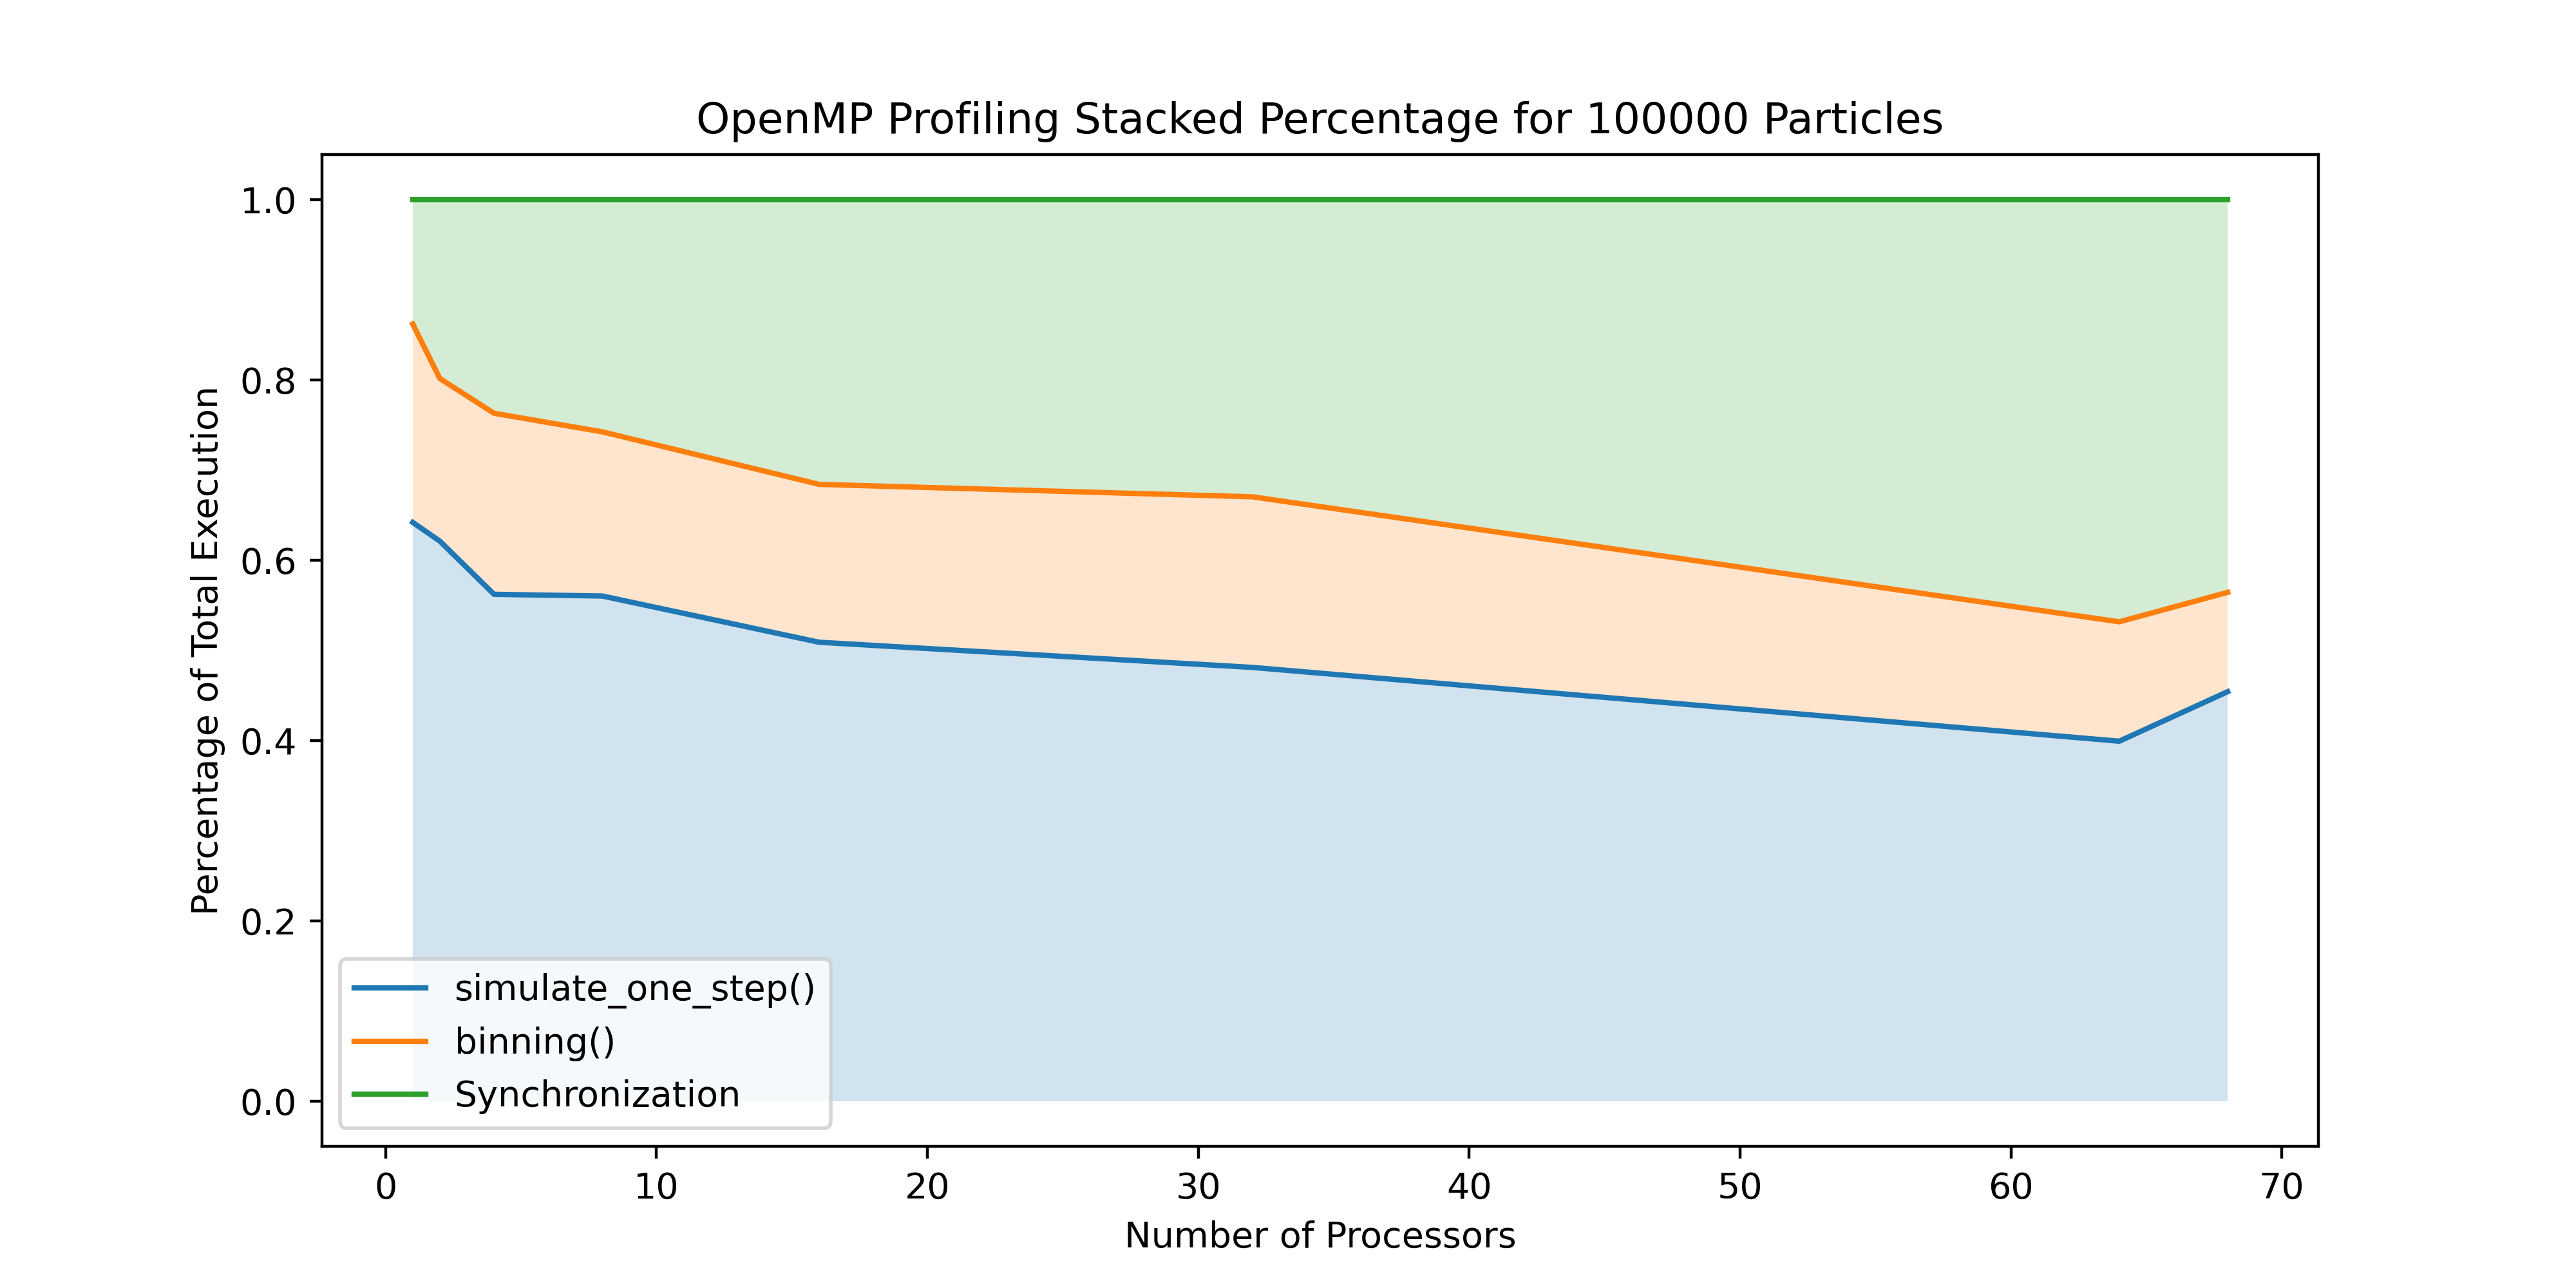
\includegraphics[width=6in]{figures/openmp_profiling_stacked_percentage.png}
\caption{OpenMP Performance Breakdown Stacked Percentage}
\label{fig:openmp-profile-stacked-percentage}
\end{figure}

We see that synchronization indeed takes a significant portion of the runtime. We wish to do more fine grain analysis if we were able to, because we're curious if there is any load imbalance between the bins that causes this significant portion of synchronization. But fortunately, we see that the percentage the simulation spends in computing, under \verb|simulate_one_step()| and \verb|binning|, ranges between 60-85\%. 

\section{Can We Do Better?}
Future possible optimizations include prefetching, and finding a smaller bin size to use. This is to exploit cache locality since a thread/core will share L1 and L2 cache. Lower levels of the memory hierarchy like L3 and main memory are shared amongst cores. If we wanted, we could also exploit DLP (data level parallelism) with the use of SIMD. This type of optimization is much harder to do since we're working with classes and data is not necessary tightly packed and DLP friendly like the data in our matrix multiplication homework. Compared the the TLP (thread level parallelism) that KNL node provides (68 cores/272 threads), it's a much easier optimization to achieve speedup with purely MIMD. Finally, it's possible we used more synchronization than necessary for correctness. For instance, a few barriers and locks could possibly be removed if done correctly and we could've resorted to using atomics instead. 

We think we will be able to improve the $p$-times speedup by removing synchronization, because the synchronization will cause a significant amount of usage of time based on our performance. And it will help, because synchronization stalls code to enter critical section. As we see from our performance breakdown, there is a lot of overhead that can be brought down with improving synchronization.

We also could've tried to utilize FMA, as there are some multiply accumulates. This can theoretically increase our performance $2\times$. But because we were tested on correctness against an implementation that didn't use any FMAs, we didn't utilize it. FMAs can provide more accurate precision since it does one rounding instead of two on separate multiply and add. But since a small precision error can deviate the final answer by a lot, it was not feasible to implement in order to pass the correctness checks.

In order to theoretically determine if we can do better, we also counted the number of FLOPs (floating point operations) to compute the FLOPS (floating point operations per second). This will determine if we are near peak performance or the theoretical peak of the KNL processor. 

The derivation of theoretical peak will be slightly different than the ones we were given in our previous homework. This is because we are not utilizing any SIMD instructions or utilizing FMA, which can increase the peak performance by $16\times$. 

Thus, our theoretical peak for this simulation can be defined as:

$$\frac{1.4 \times 10^9 \textrm{ instructions}}{\textrm{second}} * 68 \textrm{ cores} = 95.2 \textrm{ GFLOPS}$$

\begin{figure}[H]
\centering
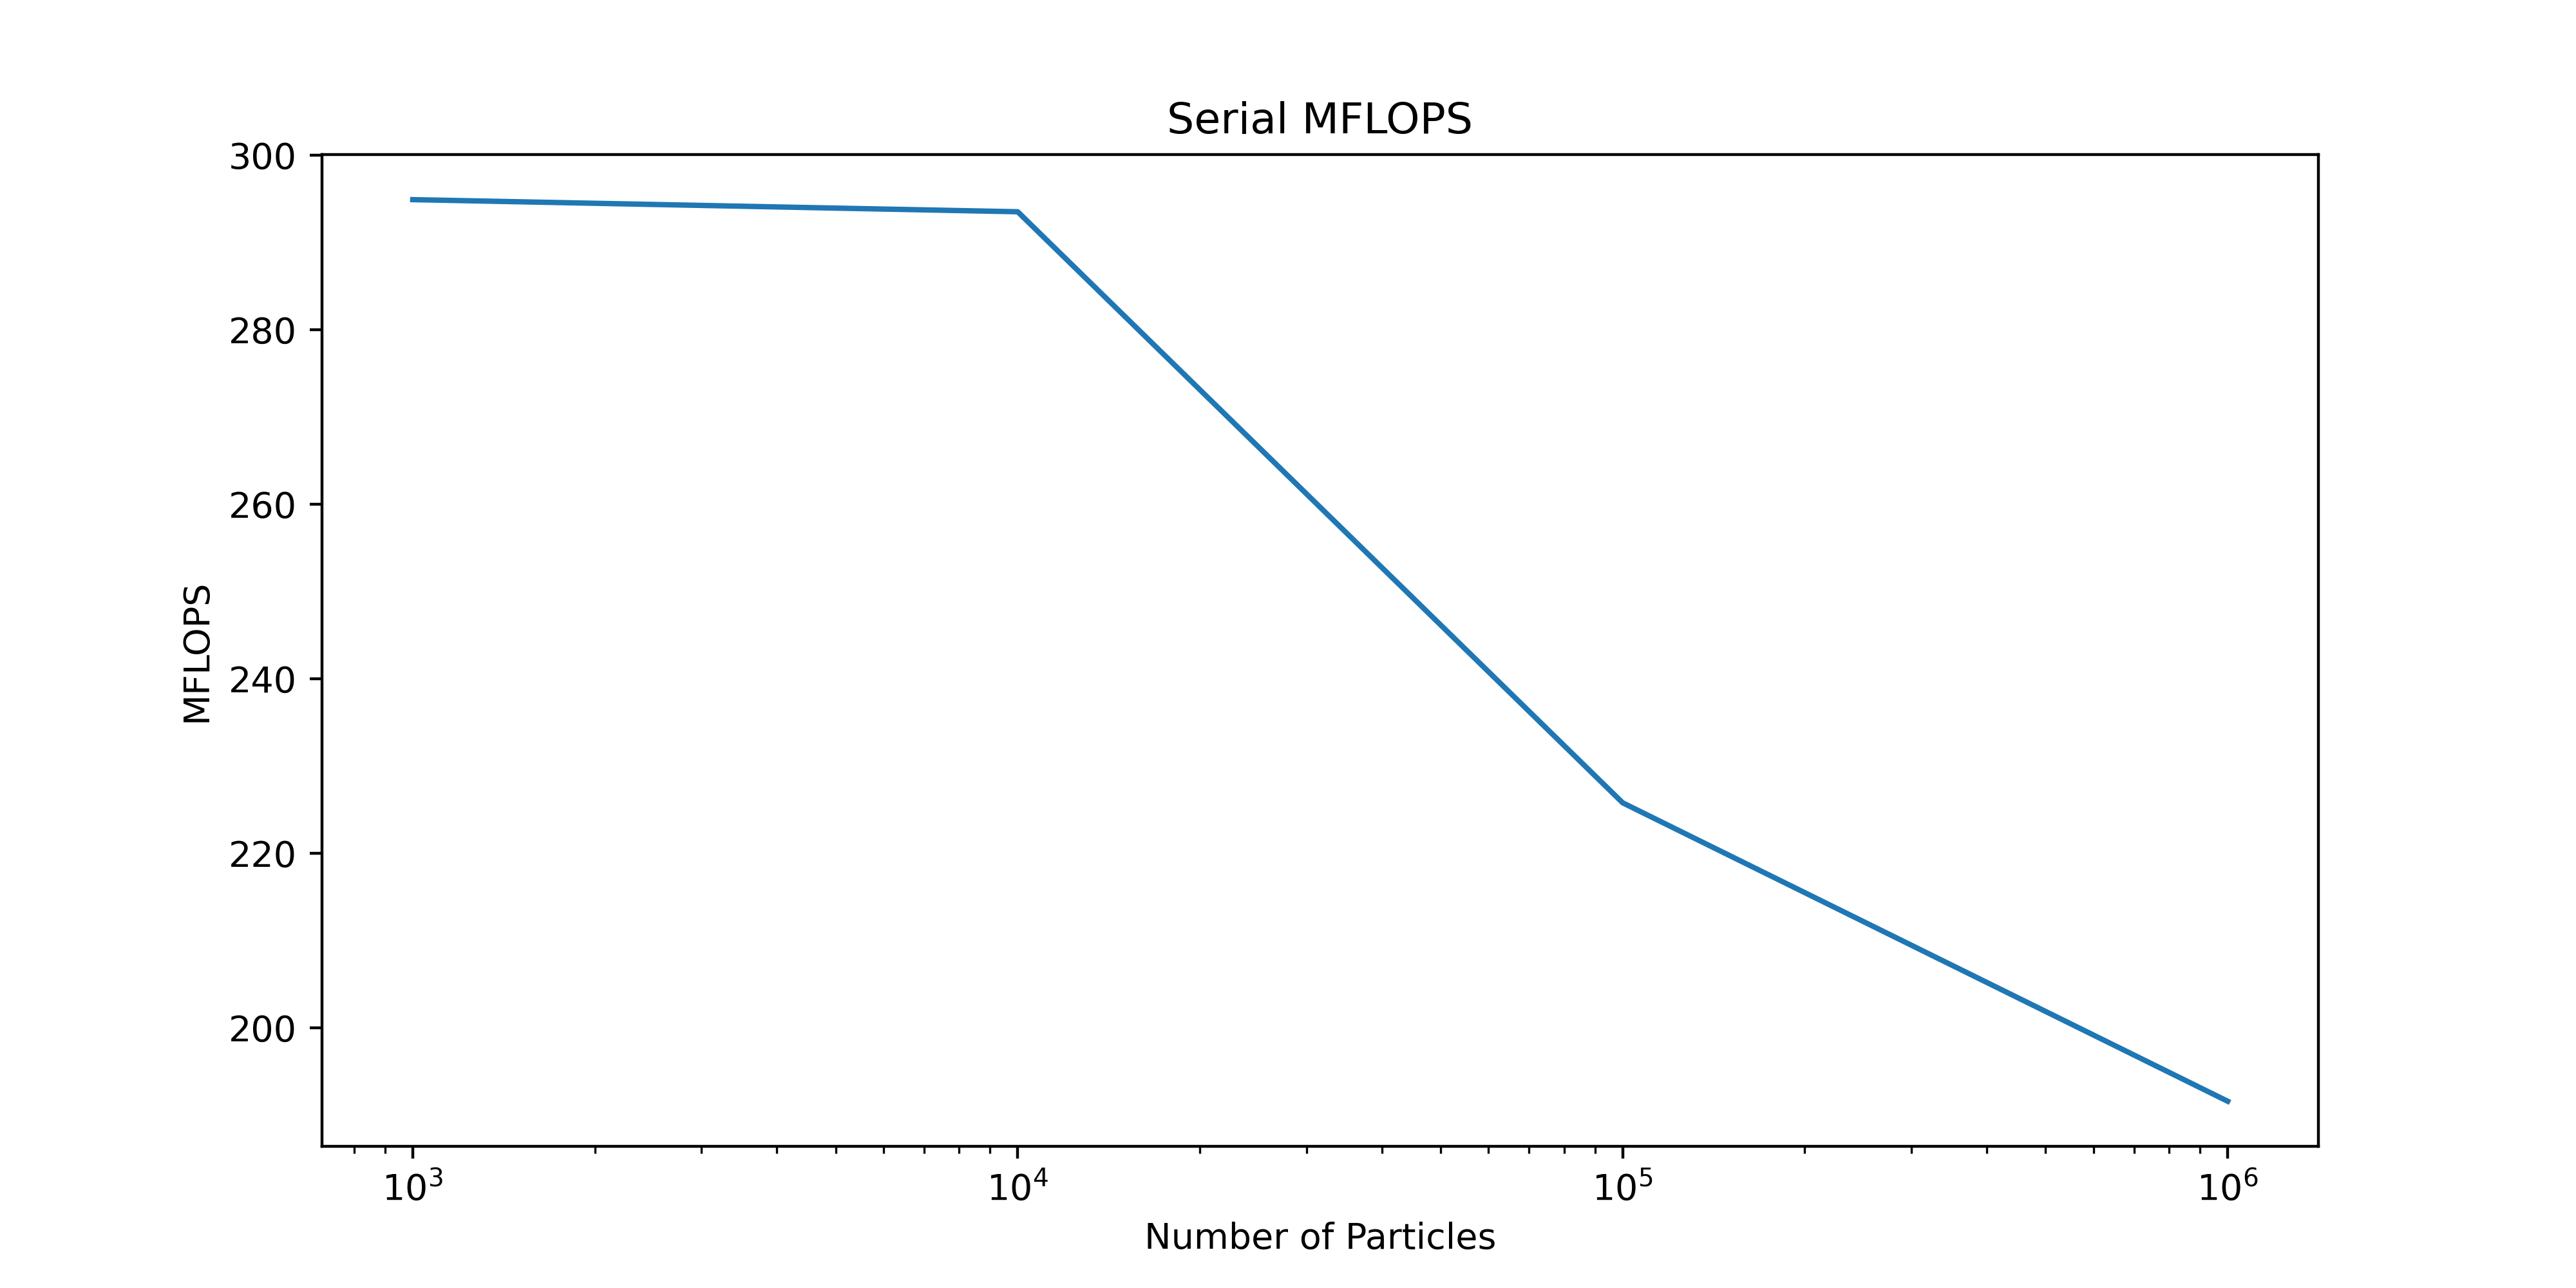
\includegraphics[width=6in]{figures/serial_flops.png}
\caption{Serial MFLOPS}
\label{fig:serial-flops}
\end{figure}

We counted the number of FLOPs by counting the number of operations manually on the serial version of the code. Figure \ref{fig:serial-flops} shows the performance. We see that performance drops off, indicating that particles don't fit in cache anymore and we suffer from increased memory accesses with larger number of particles. We hit a peak of 294.87 MFLOPS.

\begin{figure}[H]
\centering
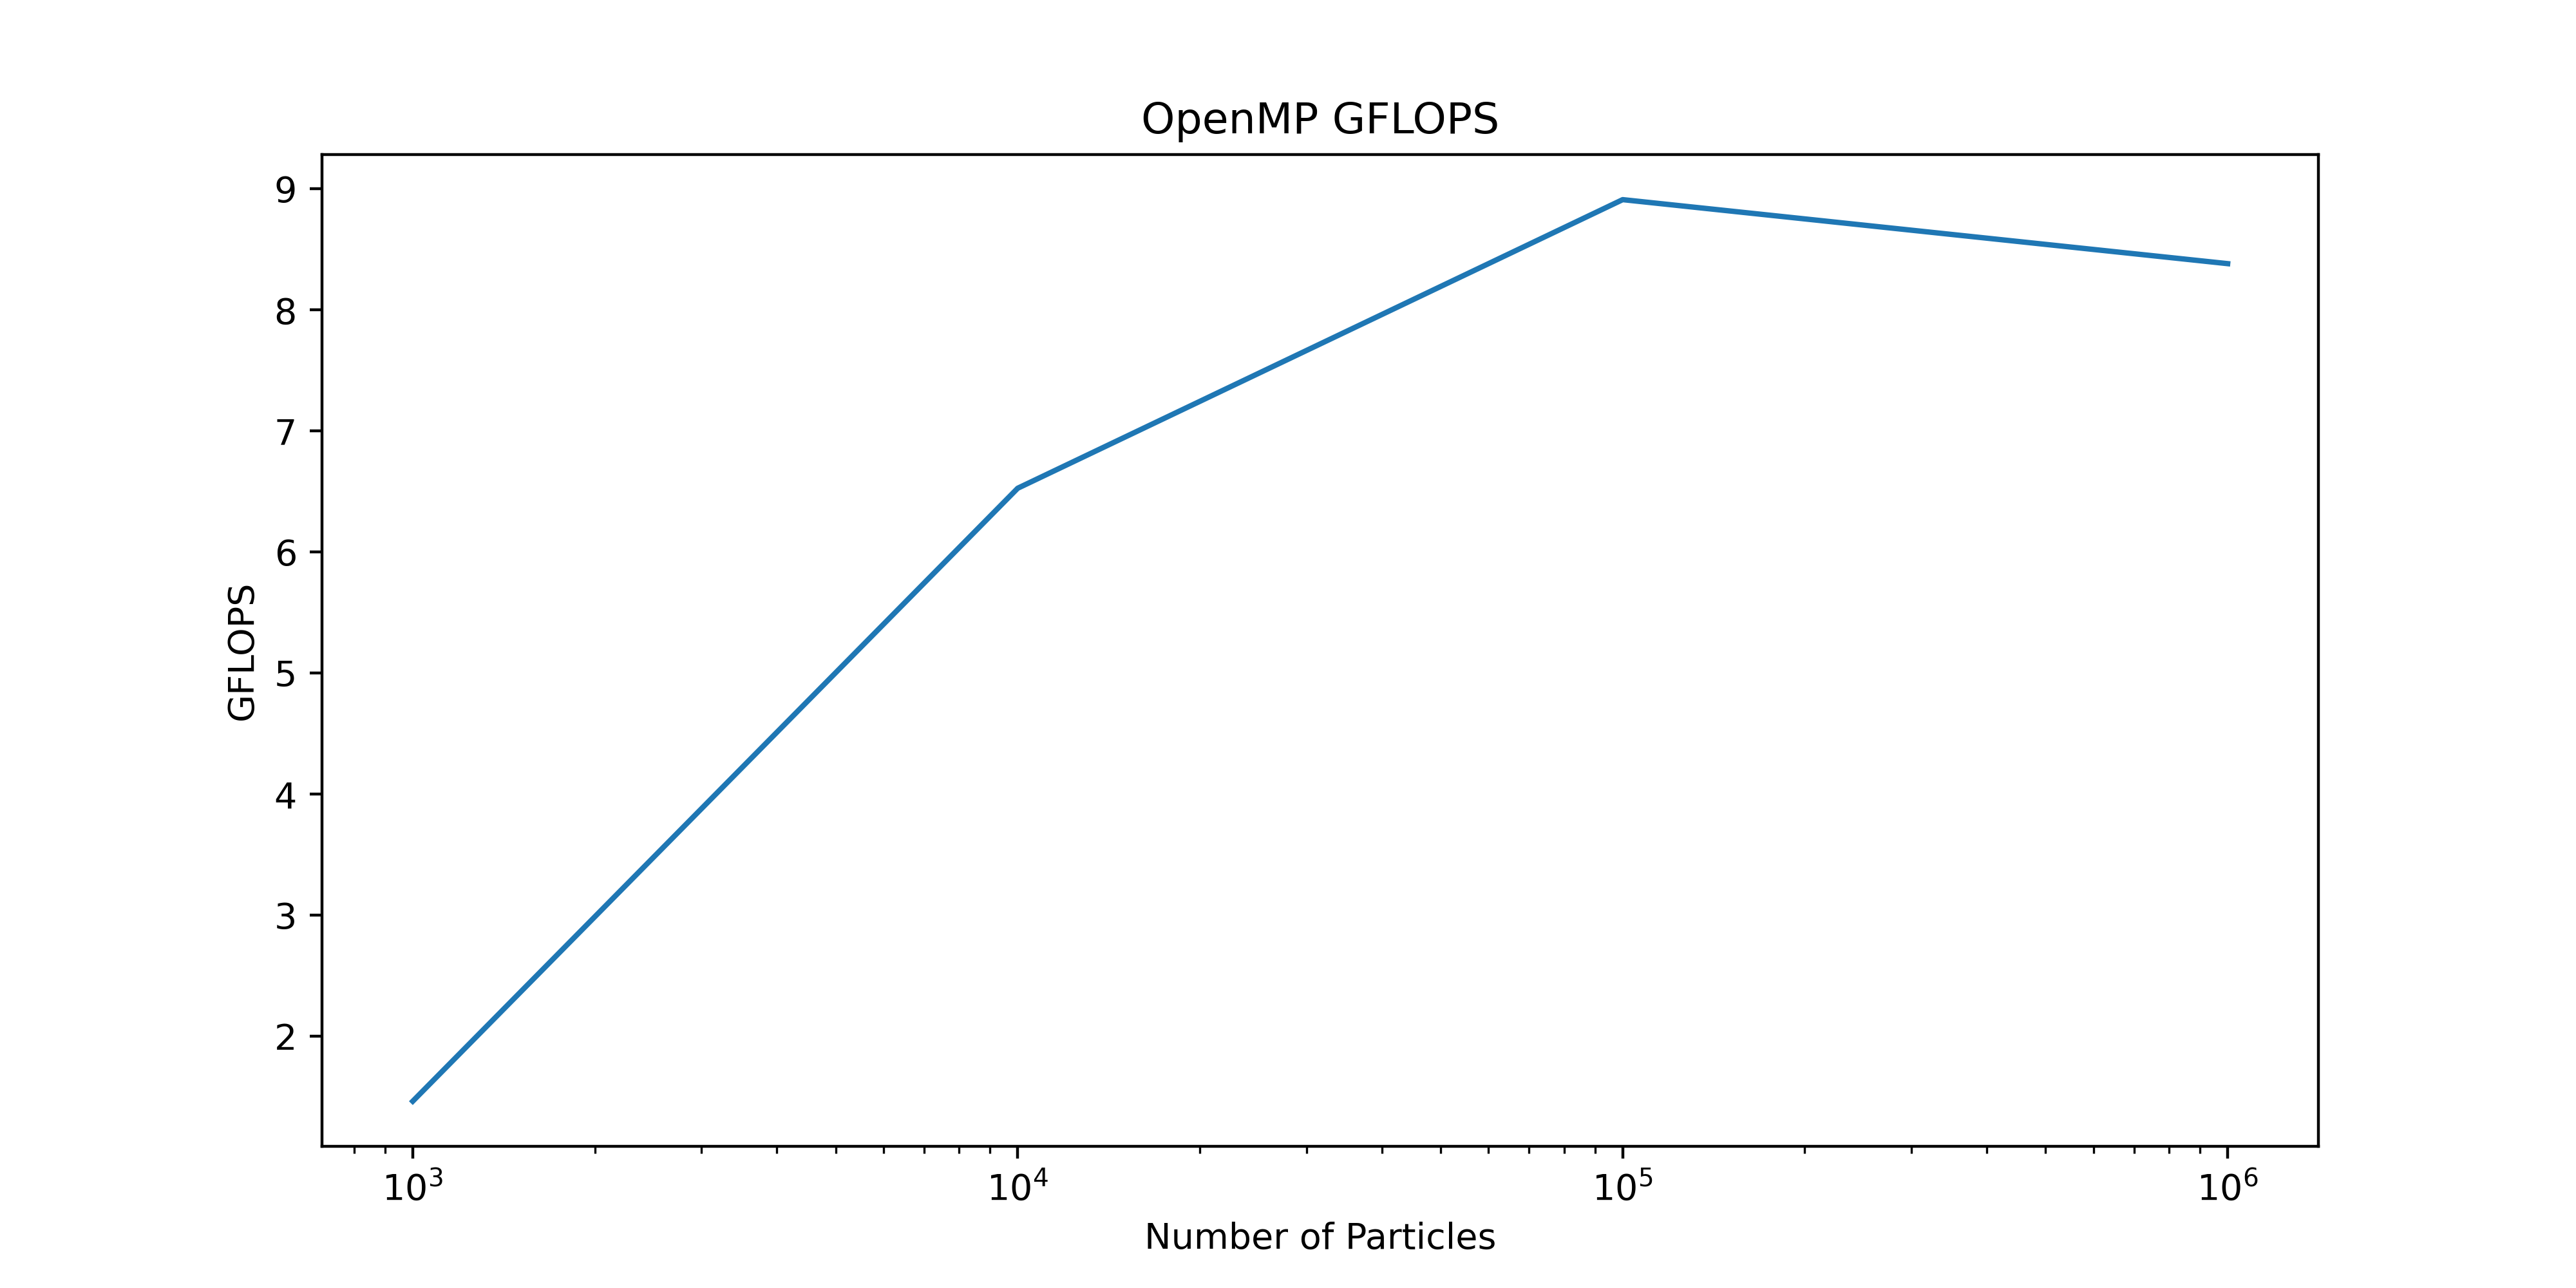
\includegraphics[width=6in]{figures/openmp_flops.png}
\caption{OpenMP GFLOPS}
\label{fig:openmp-flops}
\end{figure}

We reach a peak of 8.9120 GFLOPS when running simulations with OpenMP. Thus, our solution reaches 9.36\% of the theoretical peak. This number is embarassingly low, but understandable. The key to reaching high compute intensity is to hide latencies, especially with memory. Because our code contains a lot of memory management, such as binning and accessing data structures through pointer chasing, we are memory bounded. In order to reach higher performance, careful rethinking of how to design the algorithm and memory management must be considered.

\section{Contributions}
Xuan started off with implementation of particle binning to reduce the time complexity to $O(n)$. Brian was able to figure out an algorithmic way to speed up serial performance by reducing the number of comparisons per each iteration in a bin. Andrew was able to speed up Brian's implementation even more to a record time of 876.9 seconds (1 million particles) with a few more optimizations related to memory management. For OpenMP, Xuan and Brian was able to figure out how to add OpenMP directives to optimize code. Brian figured out how to parallelize the code as much as possible, as well as adding locks and synchronization primitives to ensure correctness.

\bibliographystyle{ieeetr}
\bibliography{references} 
\end{document}
